\documentclass[12pt]{article}
\usepackage[utf8]{inputenc}
\usepackage[margin=1in]{geometry}
\usepackage{graphicx}
\usepackage{titling}
\usepackage{setspace}
\usepackage{fancyvrb}
\DefineVerbatimEnvironment{Code}{BVerbatim}{baseline=t}
\usepackage{courier}
\usepackage{float}
\usepackage{changepage}
 \usepackage{indentfirst}
 \usepackage[titletoc]{appendix}



%WIP Title
\title{E190AT Final Project Report:\\%
       \textbf{Harvey Mudd Miniature Machine Minified}}
\author{Erik Meike, Caleb Norfleet, and Kaveh Pezeshki }
\date{April 2019}

\pretitle{%
  \begin{center}
  \LARGE
  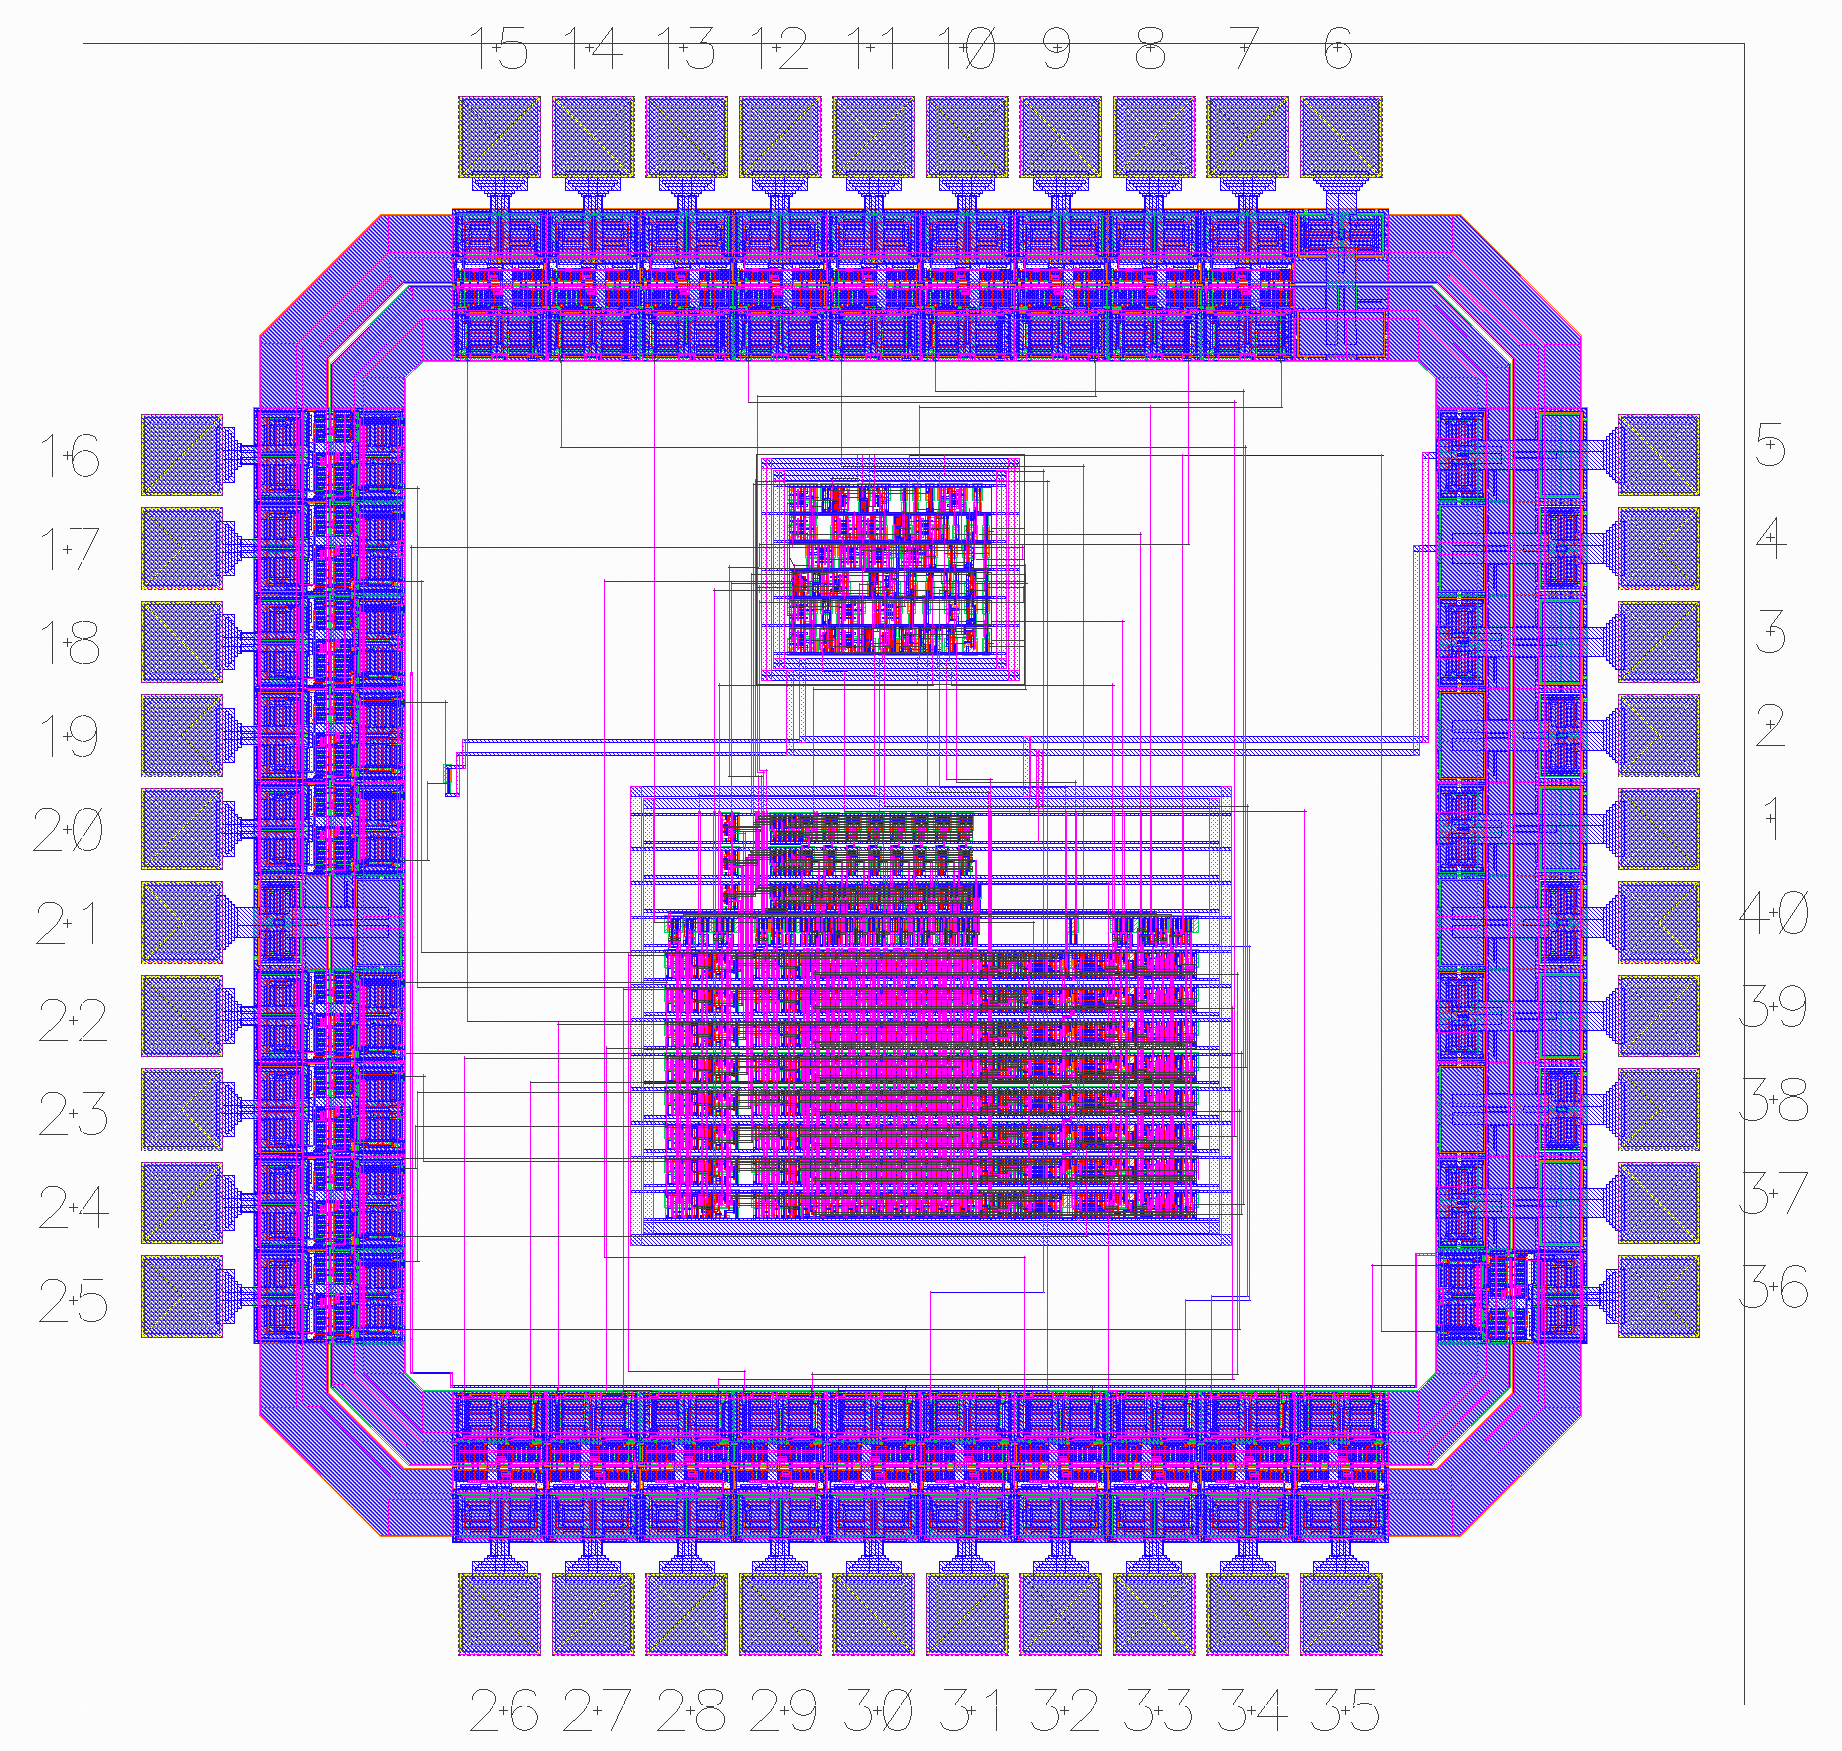
\includegraphics[width=15cm]{HMMChip.png}\\[\bigskipamount]
  \par\noindent\rule{\textwidth}{0.4pt}
  }
\posttitle{\end{center}}

\begin{document}

\maketitle
\thispagestyle{empty}
\clearpage
\setstretch{1.2}

\section{Introduction}

CSCI005, Introduction to Computer Science, and CSCI042, Principles and Practice of Computer Science, teach many Harvey Mudd freshman low-level computer architecture through the Harvey Mudd Miniature Machine (HMMM) ISA (``Documentation for HMMM"). While the HMMM ISA provides an effective tool to learn assembly language, it can be difficult for students to connect the Python HMMM simulator to the physical computers they interact with daily.

This report presents a physical implementation of a subset of the HMMM ISA which we have named the Harvey Mudd Miniature Machine Minified (HMMMM), designed for the 0.6$\mu m$ MOSIS process ($\lambda=0.3\mu m$) on a 1.5$\times$1.5mm die. We hope that a phyical implementation of the HMMM ISA will help connect high-level computer science concepts to real-world devices.

HMMMM implements a 15-bit-instruction dual-cycle CPU, which operates on 8-bit data words. The processor requires an external SRAM, as shared instruction and data memory, accessed over an 8-bit address bus. In the context of a larger system, users will be able to program the system through an external bank of switches.

\section{HMMMM Design}

\subsection{Overall Architecture}

HMMMM is a simple 15-bit-instruction, 8-bit-word processor, with eight general purpose registers. The supported instruction set is described in Figure 1. In order to simplify the shared instruction and data memory without a pipelined multicycled architecture, instructions take two cycles to execute (with branch instructions, which only require one cycle, as an exception), allowing for separate clock cycles for instruction execution and memory write-back.

\begin{figure}[H]
    \centering
    \begin{adjustwidth}{-1cm}{}
    \begin{tabular}{ll|ccccc}
        Instruction Type & Instruction & && Encoding \\
                        &        & [14:11] & [10:8] & [7:5] & [4:2] & [1:0] \\
        Data Processing &  copy  & 0100&$<$write reg$>$&xxx&$<$read reg$>$&xx \\
        Data Processing &  add   & 0110&$<$write reg$>$&$<$read reg 1$>$&$<$read reg 2$>$&xx \\
        Data Processing &  sub   & 0111&$<$write reg$>$&$<$read reg 1$>$&$<$read reg 2$>$&xx \\
        Data Processing &  neg   & 0101&$<$write reg$>$&xxx&$<$read reg$>$&xx \\
        Memory          & loadr  & 0011&$<$data  reg$>$&xxx&$<$addr reg$>$&xx \\
        Memory          & storer & 0010&xxx&$<$data reg$>$&$<$addr reg$>$&xx \\
        Immediate       & setn   & 0001&$<$write reg$>$&$<$immediate[7:0]$>$ \\
        Branch          & jumpn  & 110x&xxx&$<$immediate[7:0]$>$ \\
        Branch          & jumpr  & 111x&$<$addr  reg$>$&xxxxxxxx \\
        Branch          & jeqzn  & 1000&$<$data  reg$>$&$<$immediate[7:0]$>$ \\
        Branch          & jneqzn & 1001&$<$data  reg$>$&$<$immediate[7:0]$>$ \\
        Branch          & jgtzn  & 1010&$<$data  reg$>$&$<$immediate[7:0]$>$ \\
        Branch          & jltzn  & 1011&$<$data  reg$>$&$<$immediate[7:0]$>$ \\
        NOP             & nop    & 0000&xxx&xxxxxxxx \\
    \end{tabular}
    \caption{The HMMMM Instruction Set. All register addresses are three bits wide.}
    \end{adjustwidth}
    \label{fig:isa}
\end{figure}

The processor exposes the 8-bit address bus, 15-bit data bus, as well as a memory write control signal for the SRAM. The SRAM is assumed to be always enabled, and is assumed to be in read mode when memory write is low.

\subsection{Datapath Design}

\begin{figure}[H]
    \begin{center}
    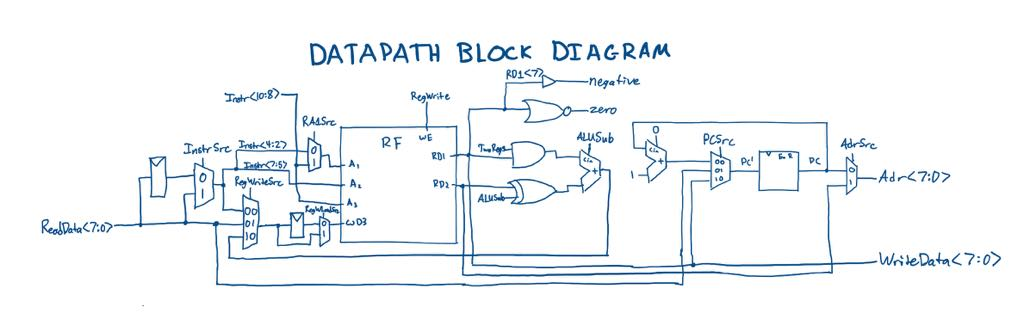
\includegraphics[width=18cm]{blockdiagram.jpg}
    \caption{Datapath Block Diagram}
    \end{center}
    \label{fig:blockdiagram}
\end{figure}

The chip is split up into two main blocks: the datapath and the controller.  The datapath, with a schematic shown in Figure 2, and HDL in Appendix A, handles the processing and routing of data, and includes the register file and the program counter.  The datapath layout is a custom block, and it is split into 12 rows.  The bottom 8 rows handle the 8-bit data stream, the top 3 rows contain the register file address decoder, and the row in between contains the zipper, where control signals are routed to the datapath from the controller.

\begin{figure}[H]
    \begin{center}
    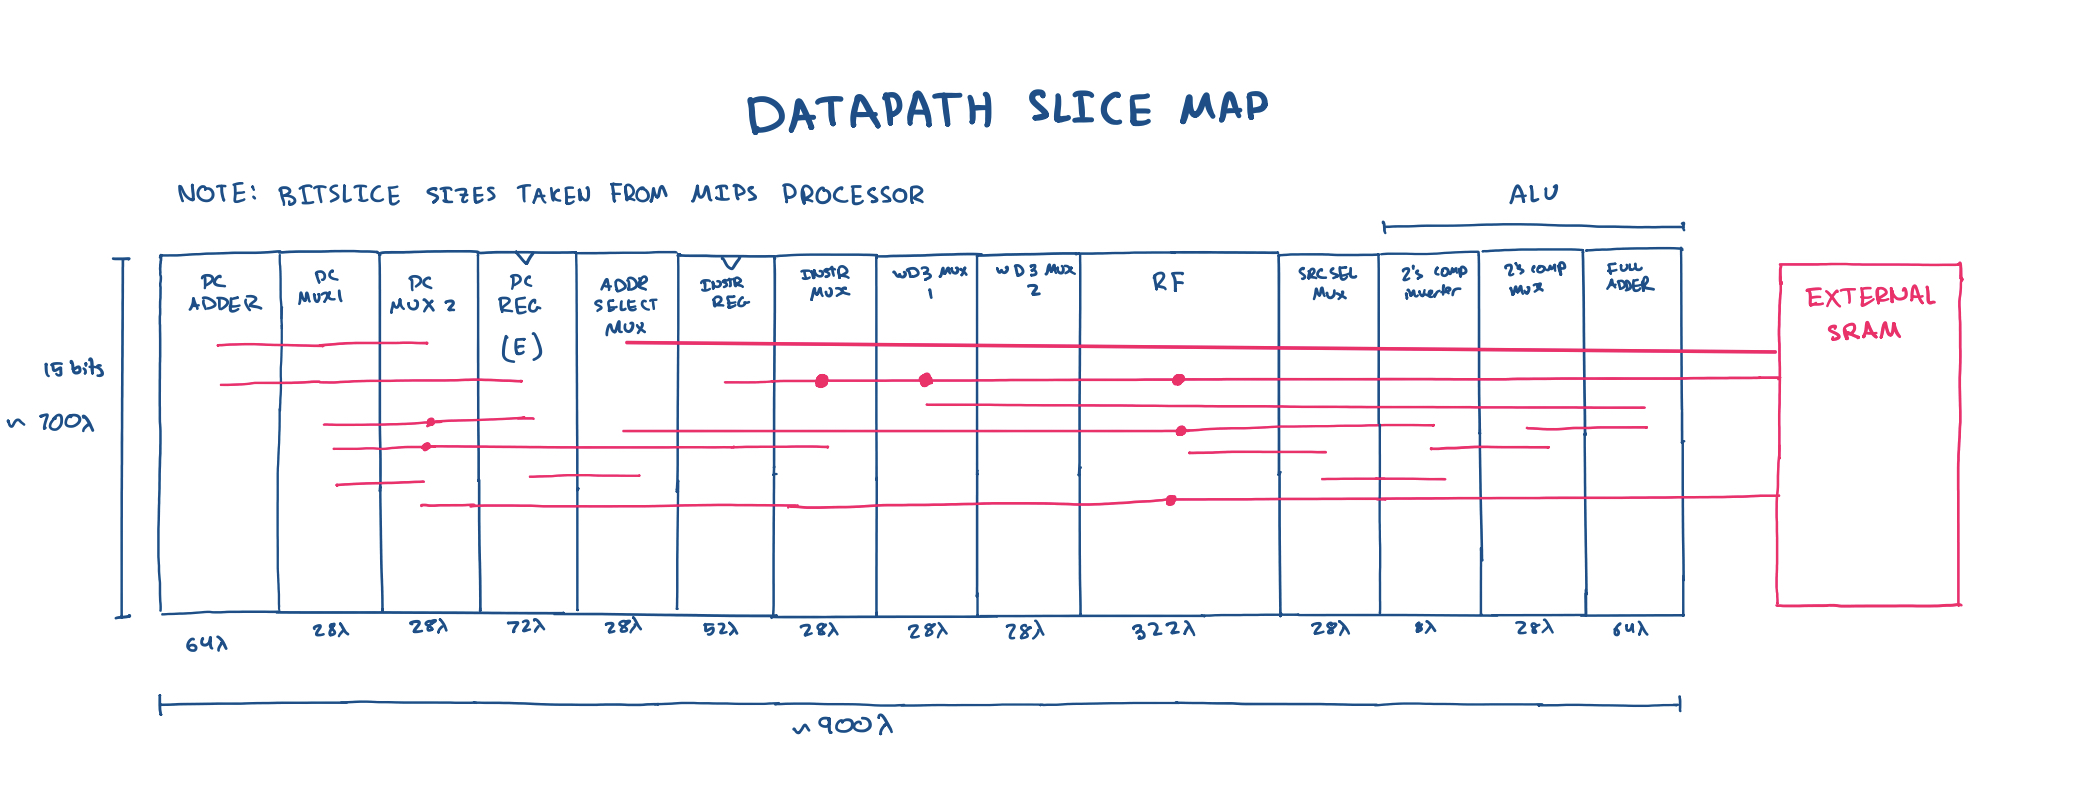
\includegraphics[width=18cm]{slicemap_old}
    \end{center}
    \caption{Proposed Datapath Slice Map}
    \label{fig:sliceplan}
\end{figure}

\begin{figure}[H]
    \begin{center}
    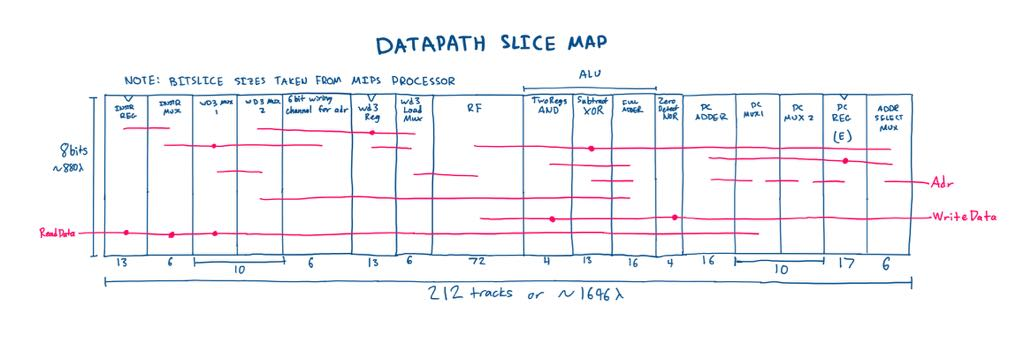
\includegraphics[width=18cm]{slicemap.jpg}
    \end{center}
    \caption{Final Datapath Slice Map}
    \label{fig:sliceplan}
\end{figure}

The slice map (Figure 3) outlines the placement of leaf cells and the routing of signals for each of the bottom 8 rows in the datapath.  By summing the width of the leaf cells one can estimate the total size of the datapath (See Figure 7 for the full chip floorplan).

%\begin{figure}[H]
%    \begin{center}
%    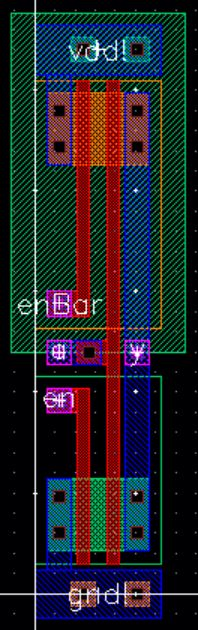
\includegraphics[width=4cm]{leafcell.JPG}
%    \caption{Tristate Inverter Leaf Cell}
%    \end{center}
%    \label{fig:leafcell}
%\end{figure}
%
%A custom tristate inverter leaf cell was created for this project.  Tristate inverters ---.  It was ultimately not used in the final layout, as the padframe was designed to integrate tristates which accomplish the intended function of these tristate inverters.

\begin{figure}[H]
    \begin{center}
    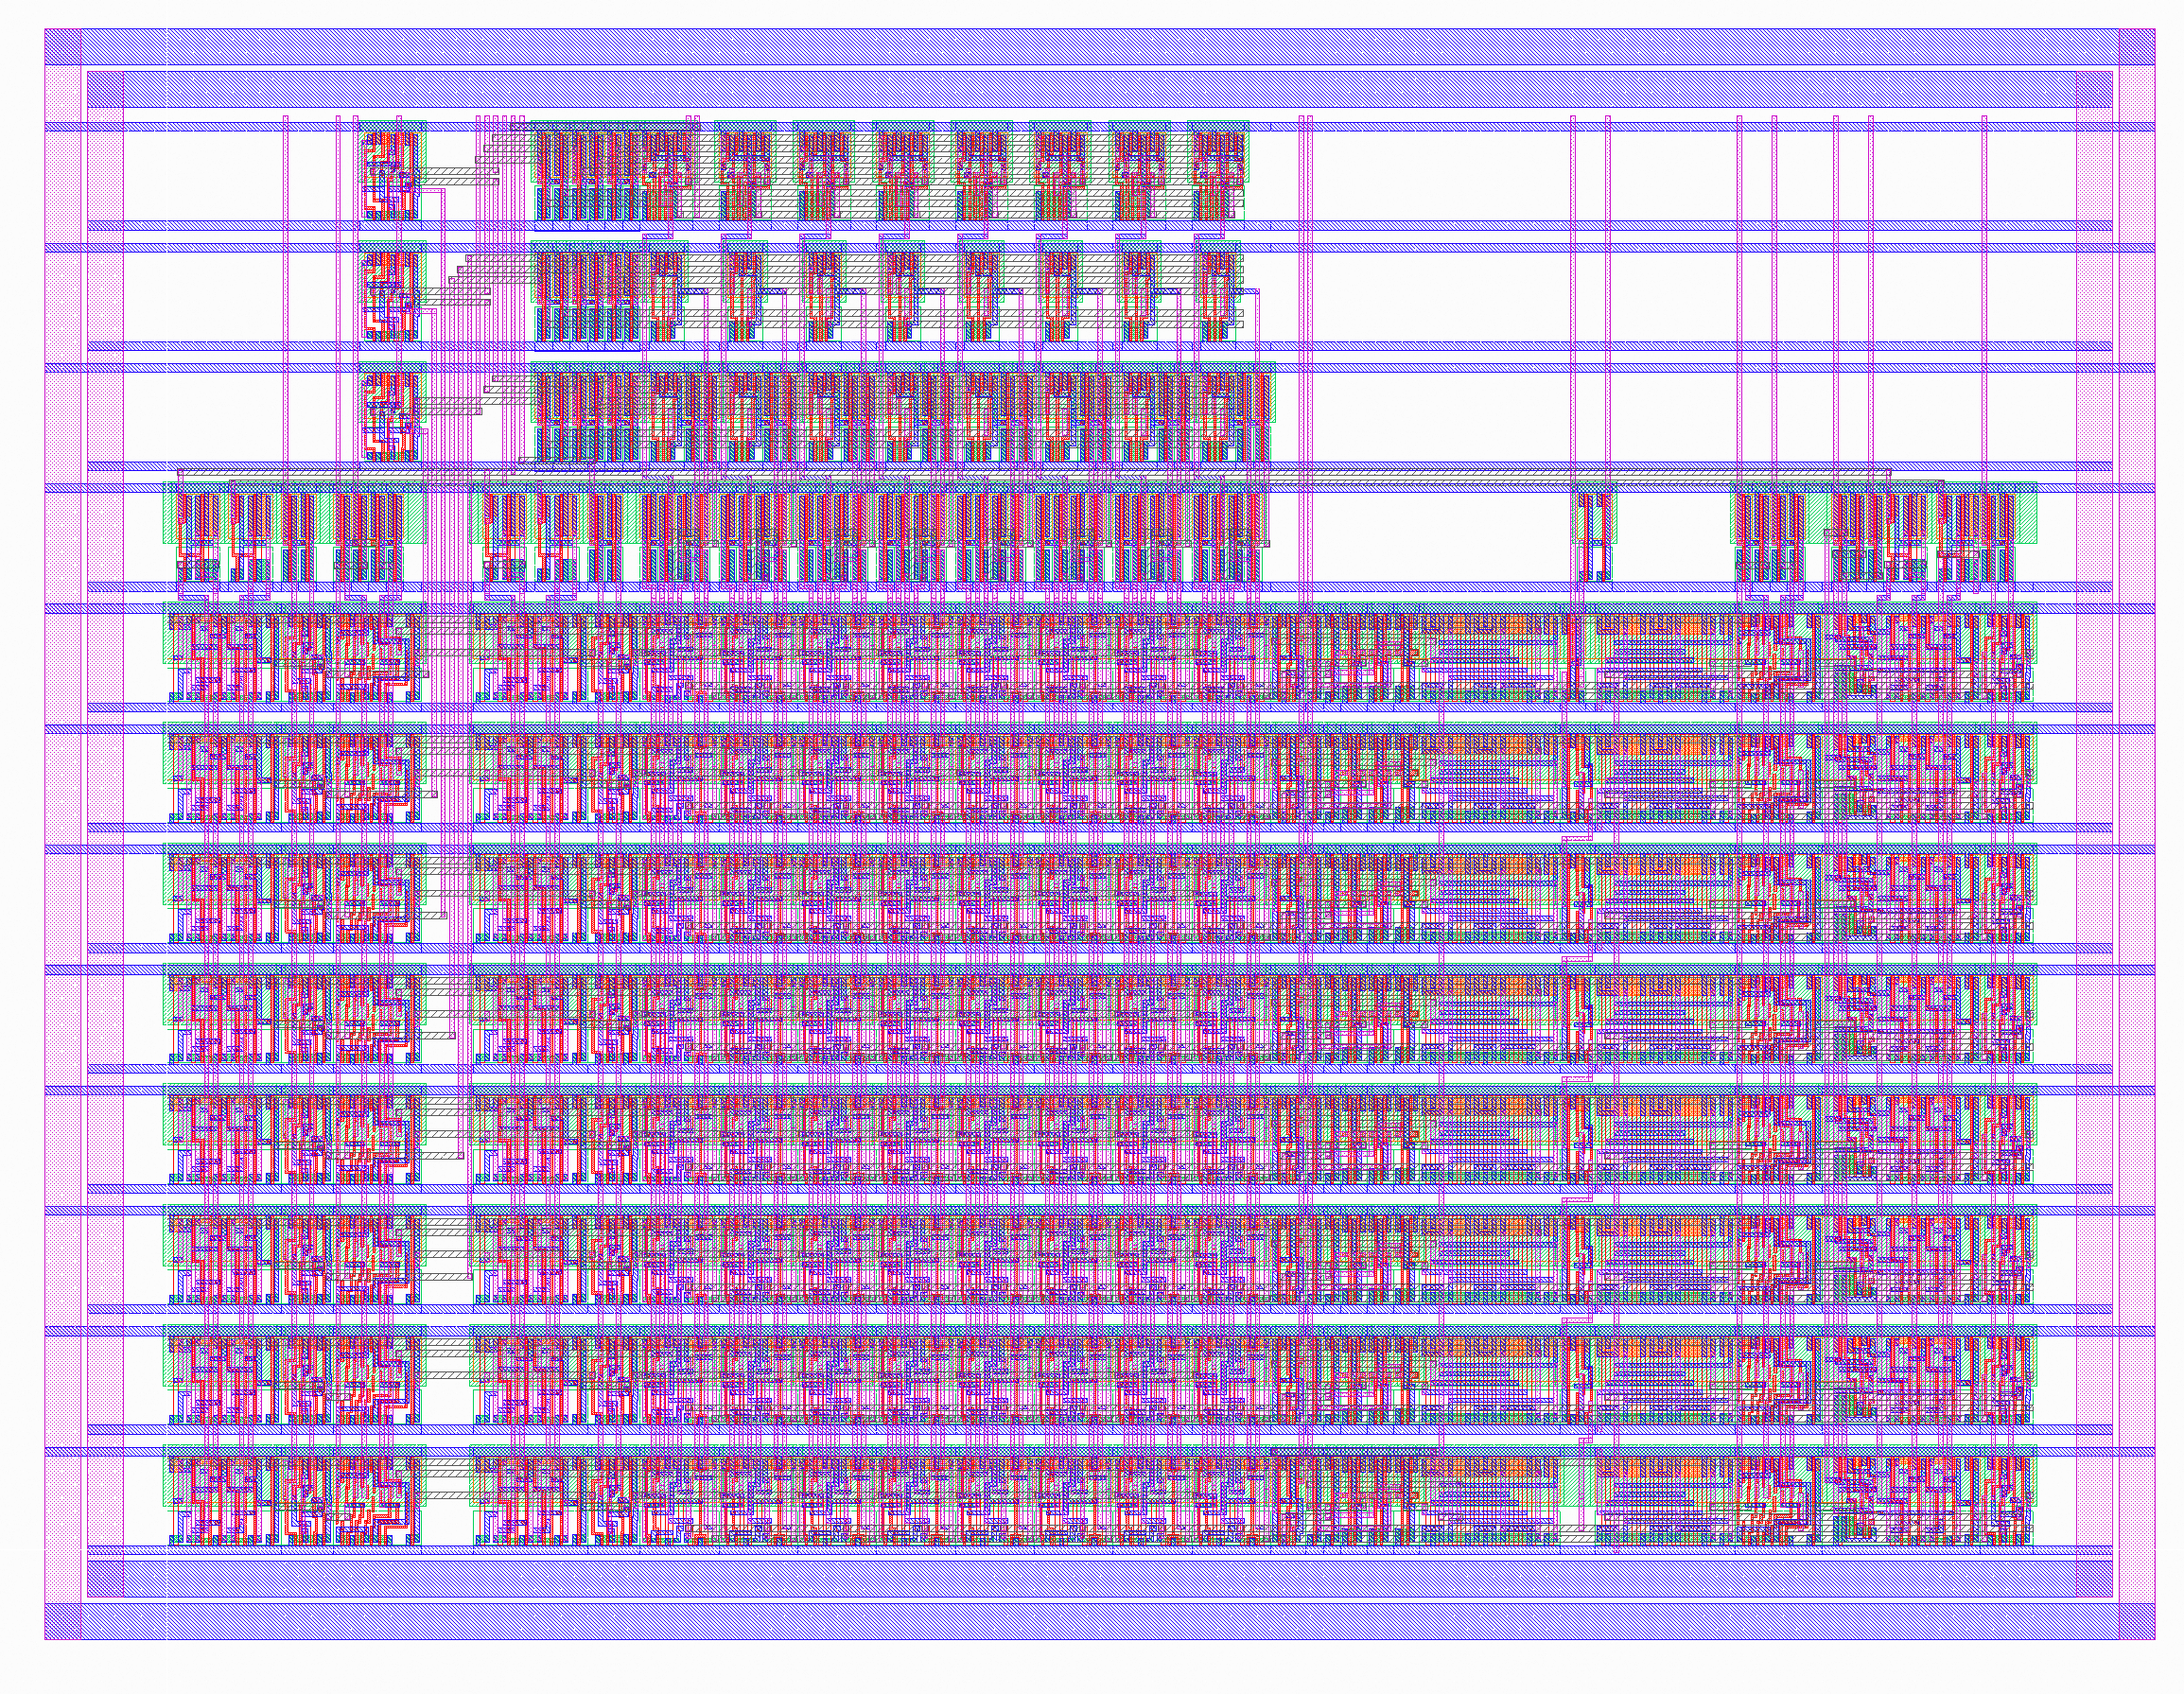
\includegraphics[width=12cm]{HMMMDatapathFull.png}
    \end{center}
    \caption{The datapath layout. A version with labelled cells is available in Appendix E.2.}
    \label{fig:datapathlayout}
\end{figure}

\subsection{Controller Design}

The controller processes an input instruction to select multiplexer and ALU modes throughout the datapath. The HDL, available in Appendix A, is synthesized into a schematic and layout.

\begin{figure}[H]
    \begin{center}
    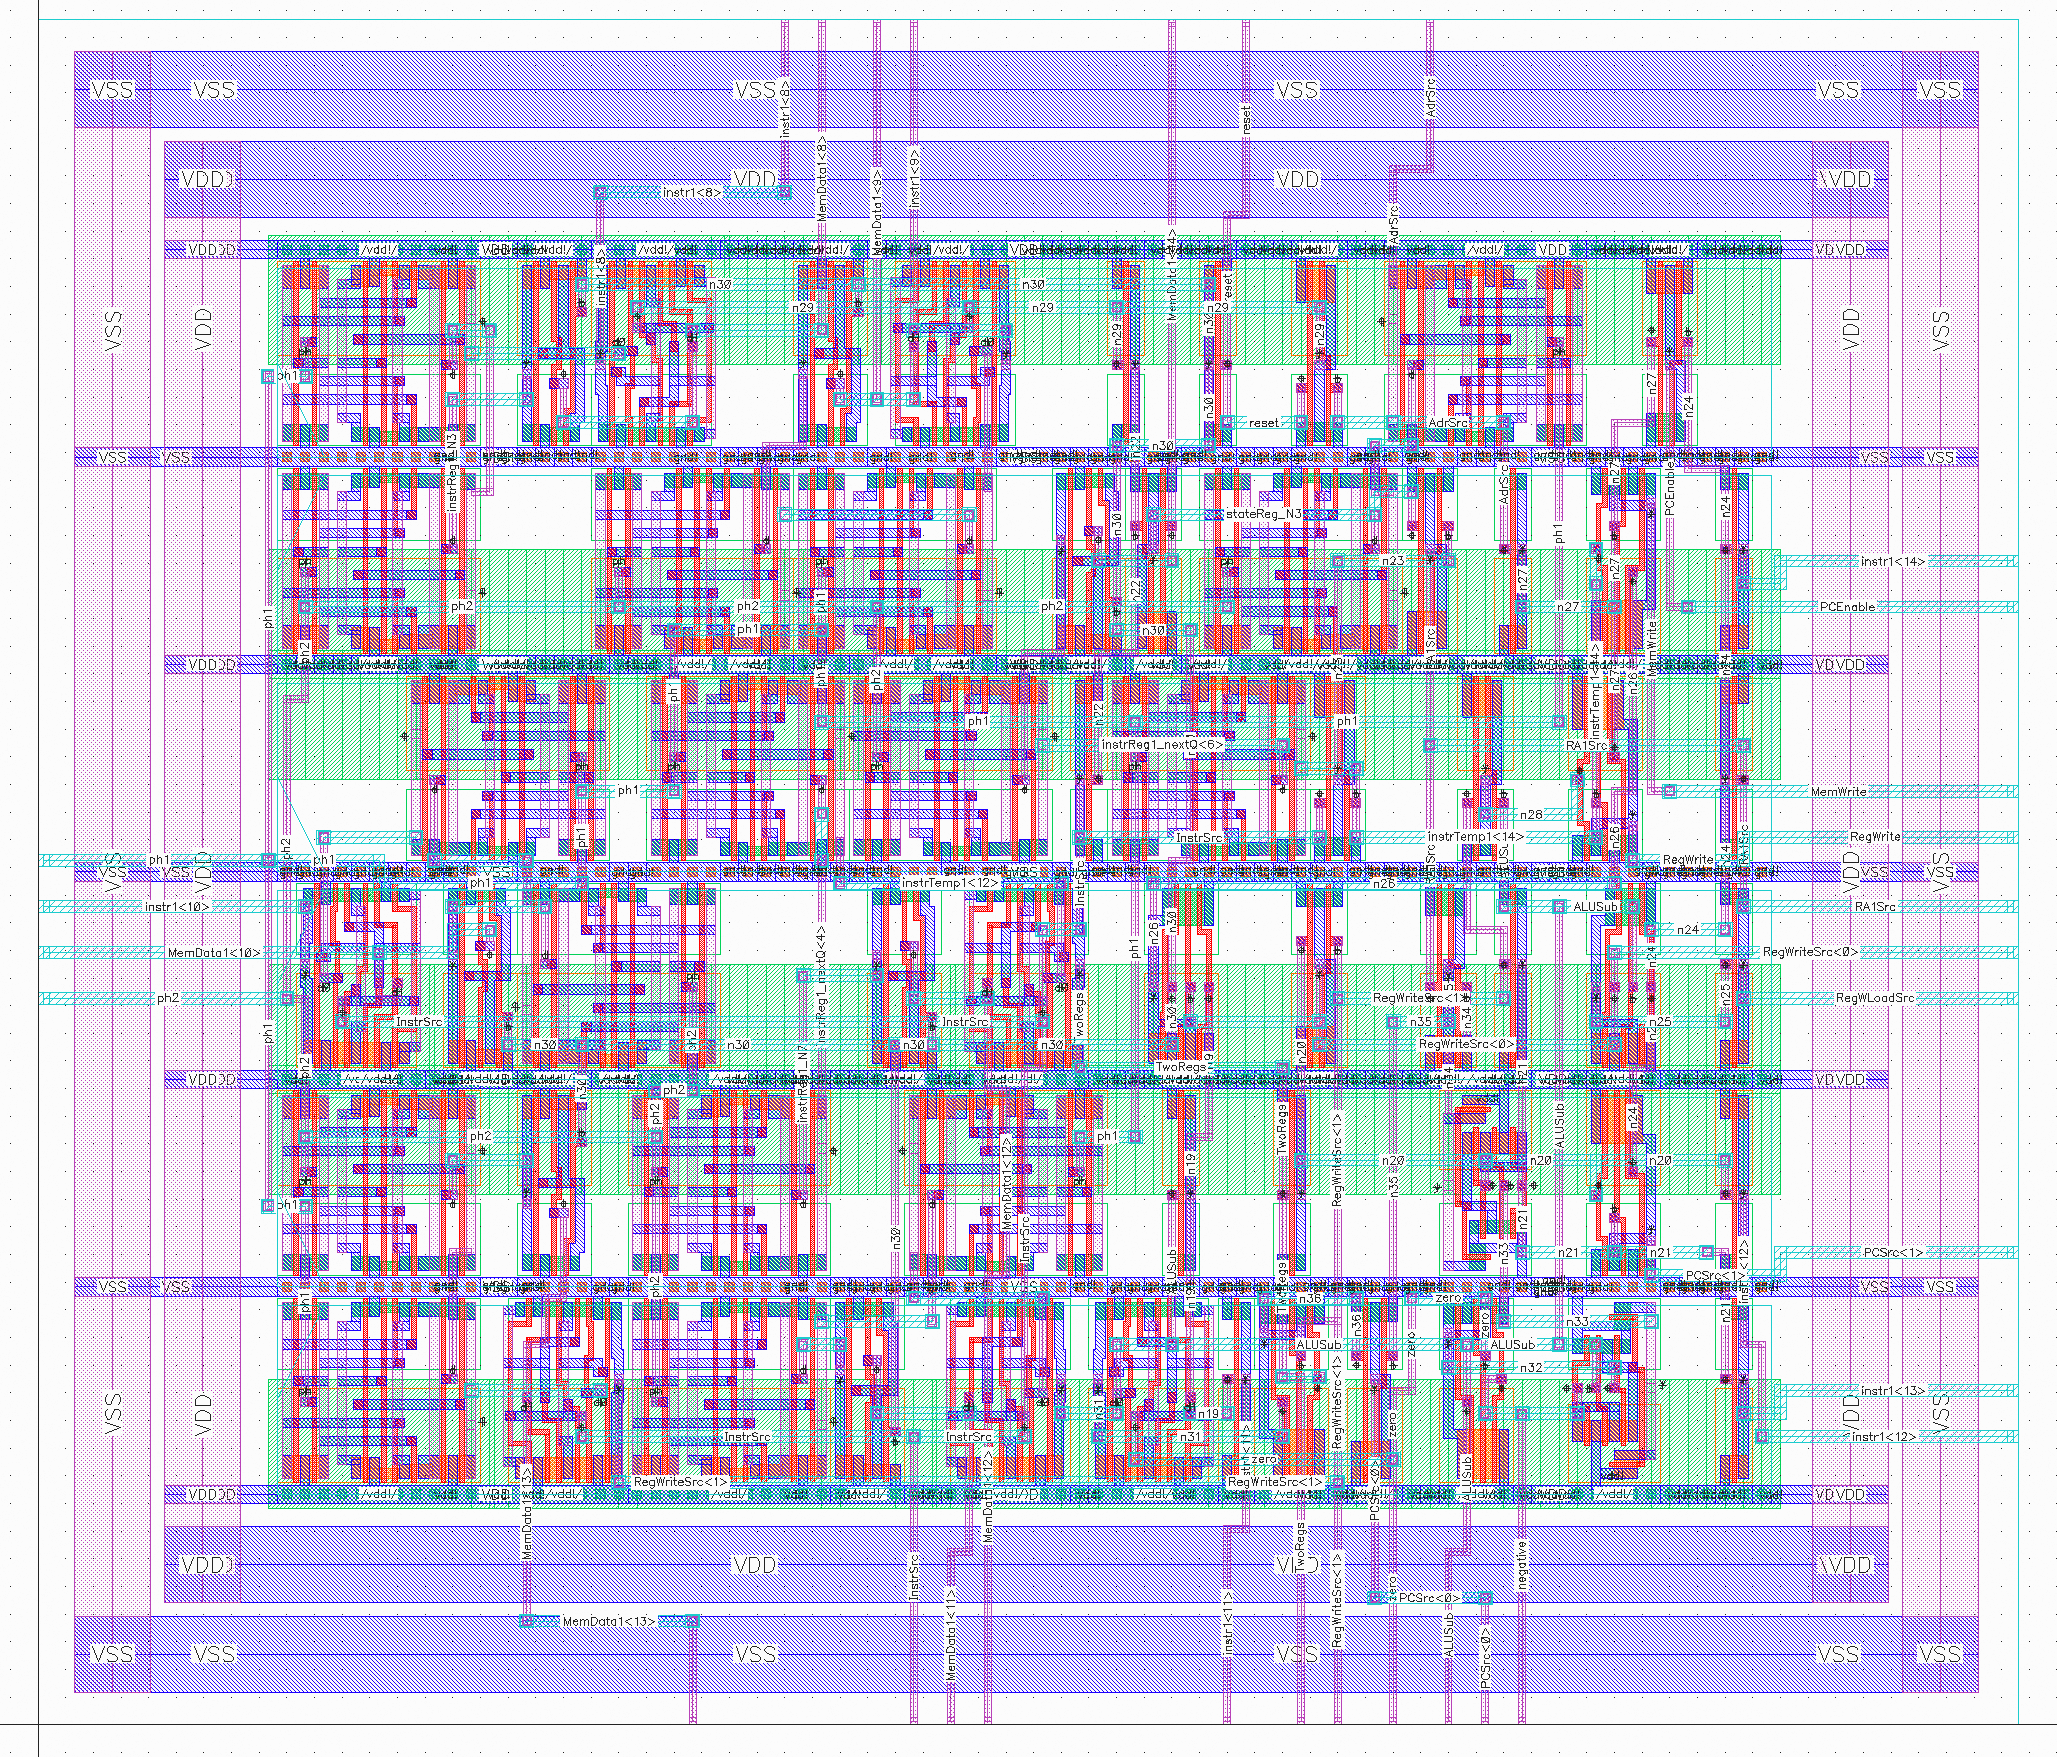
\includegraphics[width=12cm]{HMMMControllerFull.png}
    \end{center}
    \caption{The controller layout. A version with labelled cells is available in Appendix E.1.}
    \label{fig:controllerlayout}
\end{figure}

\subsection{Floorplan}

The proposed and completed floorplans are given in Figure 6 and Figure 7, respectively. Notable is a $\approx 2\times$  underestimate of datapath width in the proposed floorplan. This was due to a mis-calculation of standard cell width in the project proposal. No major changes to the datapath were made between the proposal and final layout.

This disparity is most clearly seen when examining the slice plans. The proposed and final datapath slice maps have an identical configuration, with the only difference the estimated and final width.

\begin{figure}[H]
    \begin{center}
    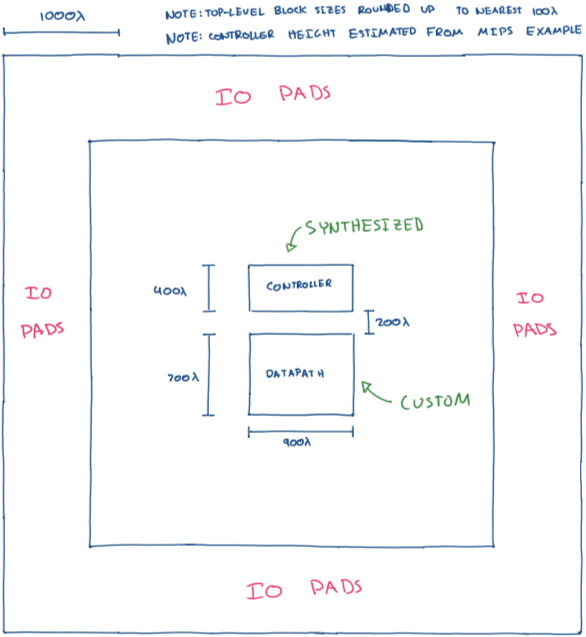
\includegraphics[width=12cm]{floorplan.png}
    \end{center}
    \caption{Proposed Floorplan}
    \label{fig:floorplan}
\end{figure}

\begin{figure}[H]
    \begin{center}
    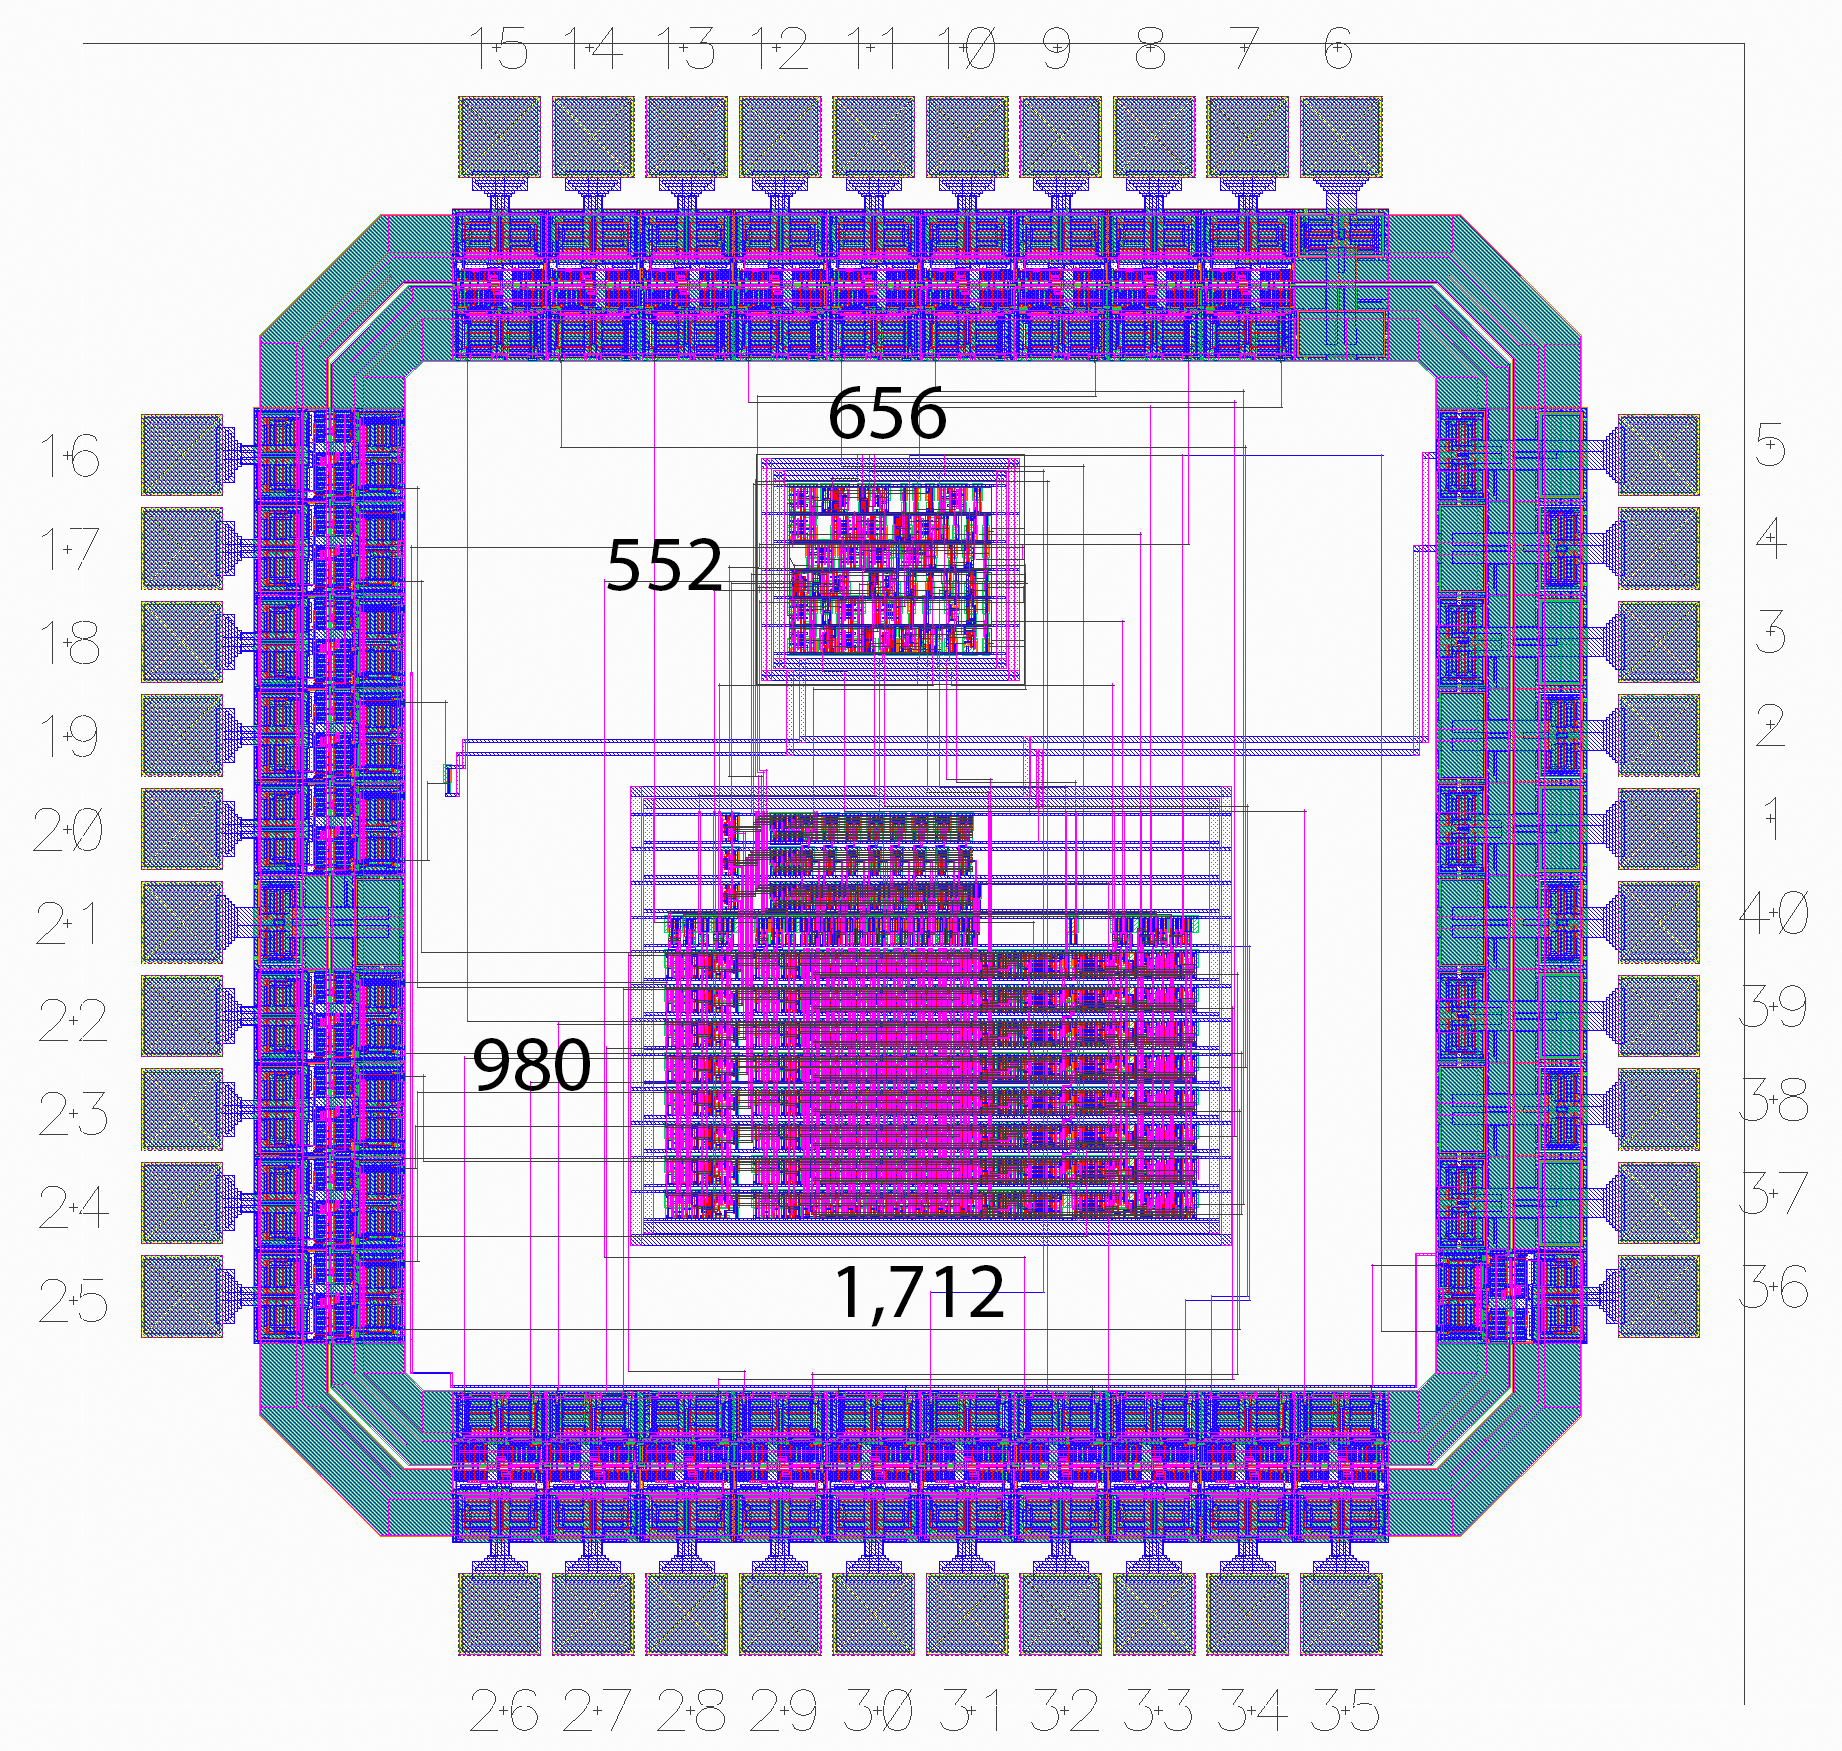
\includegraphics[width=12cm]{HMMChipLabeled.png}
    \end{center}
    \caption{Final Floorplan, Units in $\lambda$}
    \label{fig:finalfloorplan}
\end{figure}

\subsection{Pinout}

MOSIS packages the die in a 40 pin DIP. The package pinout in tabular form is provided in Figure 8. Figure 9 provides a graphical view of the device pinout. Pins 19 and 20 are tied to an inverter as a basic manufacturing test.

\begin{figure}[H]
    \begin{center}
    \begin{tabular}{lll}
        Pin Number & Pin Function & Pin Direction \\
        \hline
        1 & vdd & power \\
        2 & gnd & power \\
        3 & vdd & power \\
        4 & gnd & power \\
        5 & vdd & power \\
        6 & gnd & power \\
        7 & reset & input \\
        8 & clock phase 1 & input \\
        9 & clock phase 2 & input \\
        10-17 & address[0:7] & output \\
        18 & memwrite & output \\
        19 & test\_in & input \\
        20 & test\_out & output \\
        21 & gnd & power \\
        22-36 & memdata[0:14] & bidirectional \\
        37 & vdd & power \\
        38 & gnd & power \\
        39 & vdd & power \\
        40 & gnd & power
    \end{tabular}
    \caption{The HMMMM pinout. test\_in and test\_out are the input to and output from an inverter independent from the processor.}
    \end{center}
    \label{fig:pinout}
\end{figure}

\begin{figure}[H]
    \begin{center}
    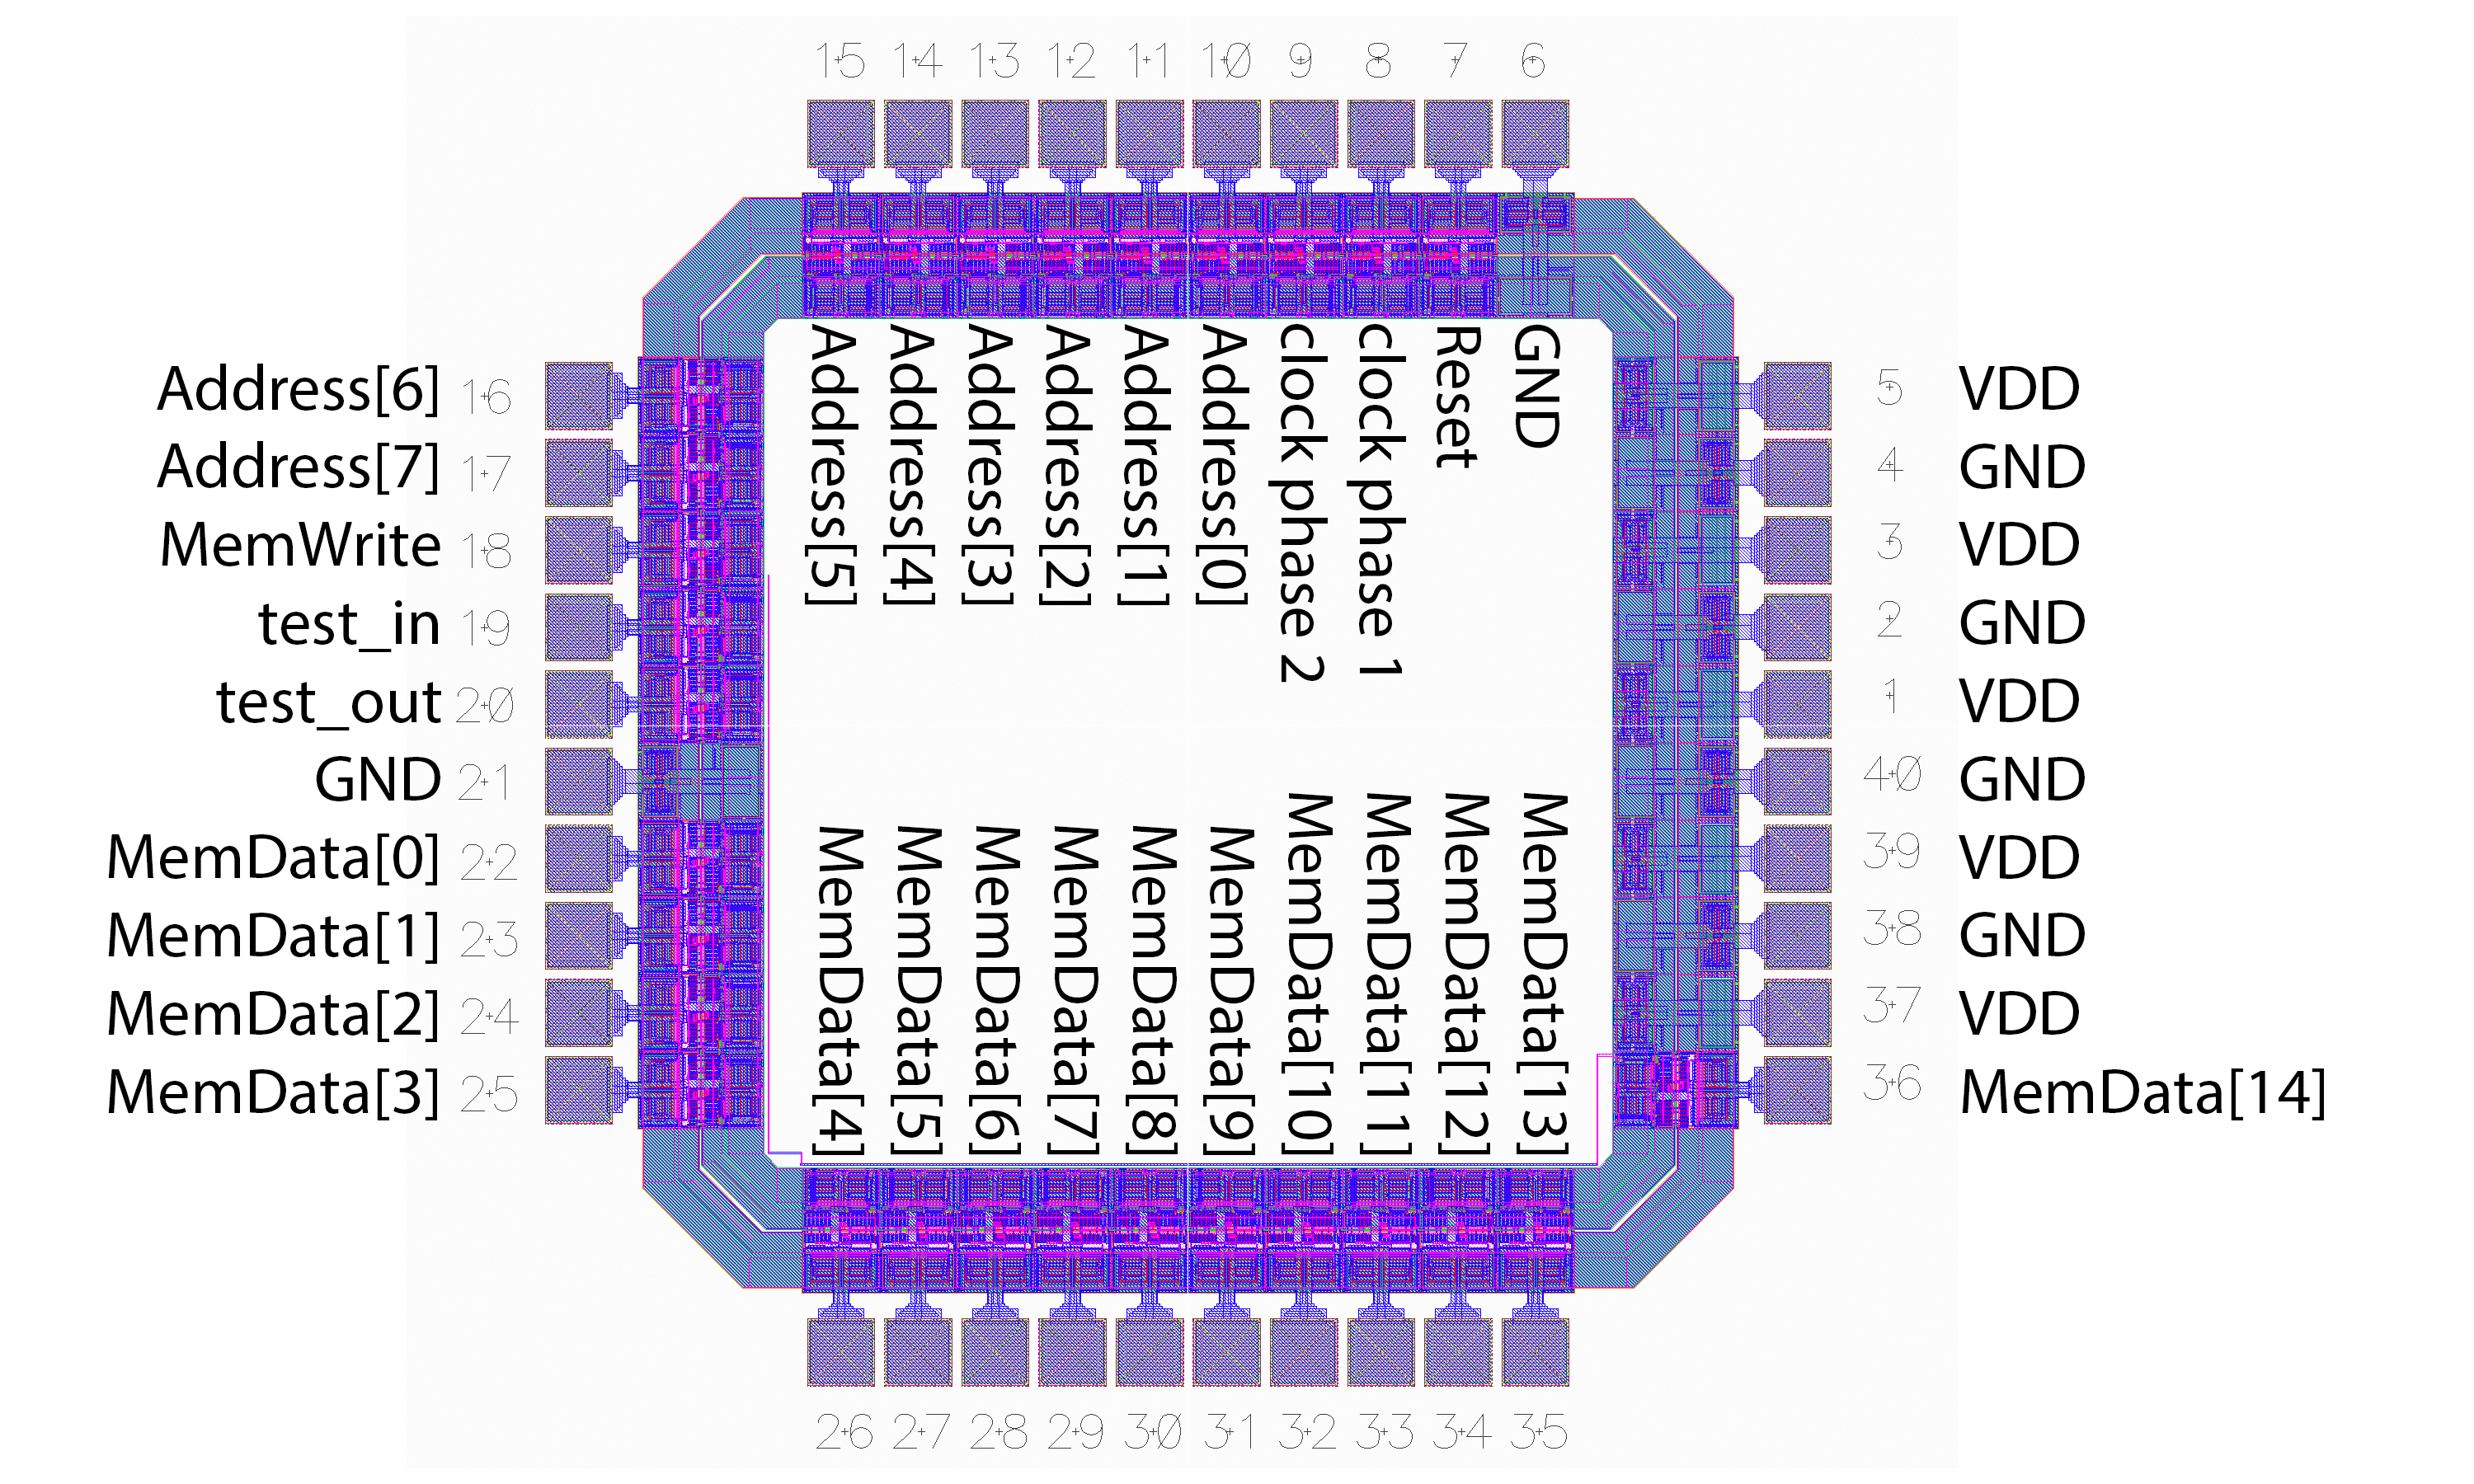
\includegraphics[width=16cm]{pinoutgraphical.png}
    \caption{A graphical view of the HMMMM pinout}
    \end{center}
    \label{fig:pinoutgraphical}
\end{figure}

\section{Verification}

The table in Figure 10 summarizes the verification status of HMMMM.

\begin{figure}[H]
    \begin{center}
    \begin{tabular}{ll}
        Verification Step & Status \\
        \hline
        HDL Passing Testbench & Complete \\
        Controller Passing DRC & Complete \\
        Controller Passing LVS & Complete \\
        Controller Passing Testbench & Complete \\
        Datapath Passing DRC & Complete \\
        Datapath Passing LVS & Complete \\
        Datapath Passing Testbench & Complete \\
        Chip Passing DRC & Complete \\
        Chip Passing LVS & Complete \\
        Chip Passing Testbench & Complete \\
        GDS Re-import & Complete \\
        GDS Verification & Complete
    \end{tabular}
    \caption{HMMMM Verification Status.}
    \end{center}
    \label{fig:verificationstatus}
\end{figure}


\subsection{HDL and Schematic Verification}

We created a self-checking SystemVerilog testbench and SRAM for controller and datapath verification\footnote{The SystemVerilog source is available in Appendix A.1 and A.2}. On simulation initialization, the SRAM loads a 32-instruction program\footnote{The testvectors are available in Appendix A.3}, and initializes address \texttt{0x40} to \texttt{0x05}. This program tests every HMMMM instruction, including less than zero, equal to zero, and greater than zero for all conditional branches.

Successful program execution will lead to the value \texttt{0x2D} written in address \texttt{0x29}. If this is not observed (i.e. if the value \texttt{0x00} appears in address \texttt{0x29}), then then the processor has malfunctioned. We substituted exported Verilog in for the controller and datapath when designing the controller and datapath schematic, and have ensured that the final design passes the testbench.

%TODO: update appendix references

\subsection{Layout Verification}

After finishing each subsection of the chip, we performed LVS (Layout Vs Schematic) by extracting the schematic from our layout automatically and then comparing this to our original schematic. This allowed us to test each cell's final functionality and isolate issues before they became harder to debug later in the design process. We performed this on each schematic level on the chip from leaf cell to the full chip. We finally exported GDS of our chip and ran LVS after re-importing the final fabrication files to ensure that no parts of the chip were broken during the export process. 

\subsection{Post-Fabrication Test Plan}

We aim to produce not just a functional chip, but a full demonstration system implementing a functional chip. This demonstration and testing system will provide:

\begin{itemize}
    \item Software-defined SRAM and processor clocks through a Lattice FPGA with onboard non-volatile configuration memory. This allows for non-volatile program storage.
    \item All HMMMM I/O accessible from 0.1" headers and tri-state buffers
    \item A digitally-controlled variable-voltage processor power supply, implemented through an LM317 and digital potentiometer
    \item A shunt resistor to measure HMMMM current requirements, and an associated ADC
    \item Low-voltage level shifters for all processor interfaces
    \item LED arrays for address and data bus visualization
    \item A switch bank for hand-programming the SRAM
\end{itemize}

Initial testing will involve loading the HMMMM program described in Section 3.1 onto the FPGA SRAM, and testing whether the physical chip correctly executes the program. If this test is successful, we will investigate the IV characteristics of the processor, including transistor response to low voltages. If this test fails, we will follow the following debugging process:

\begin{enumerate}
    \item Check resistance between vdd and gnd. A short here indicates a completely nonfunctional chip. If this occurs, we will try re-testing with another chip
    \item Check inverter behavior across test pins 19 and 20. This is a simple test of the fabrication process, and a failure here indicates a larger problem with our layout. If this occurs, we will try re-testing with another chip
    \item Debugging steps past the above points are contingent on the observed symptoms
\end{enumerate}

Finally, we will implement simple assembly programs seen in CSCI005 and CSCI042 to use the device as a demonstration tool.

\section{Logistics}

\subsection{Design Time}

The design time breakdown is illustrated in Figure 11.

\begin{figure}[H]
    \begin{center}
    \begin{tabular}{lll}
        Design Component & Design Time (Hours) & Verification Time (Hours) \\
        \hline
        Testbench HDL & 2 & 1 \\
        SRAM HDL & 1.5 & 0.5 \\
        Datapath HDL & 10 & 2 \\
        Datapath Schematic & 6 & 1.5\\
        Datapath Layout & 9 & 4 \\
        Controller HDL & 4 & 3 \\
        Controller Schematic & 7 & 2 \\
        Controller Layout & 2 & 1 \\
        Chip Schematic & 3 & 4 \\
        Chip Layout & 2 & 1\\
        Chip Export & 1 & 0.5 \\
        Leaf Cell & 1 & 0.5 \\
    \end{tabular}
    \caption{Design time breakdown for the HMMMM processor}
    \end{center}
    \label{fig:designtime}
\end{figure}

\subsection{File Locations}

All human-readable source files are included in the appendix to this report. Design and testbench HDL, as well as testvectors, are available on the project GitHub\footnote{https://github.com/VLSIProject2018/vlsi-2019}. 

Cadence design files are accessible in the repository under directory \texttt{cadence\_design\_files}. Design components are available under the following libraries and cells described in Figure 12.

\begin{figure}[H]
    \begin{center}
    \begin{tabular}{lll}
         Design Component & Library & Cell \\
         \hline
         Full Chip & HMMM & chip \\
         Chip (no padframe) & HMMM & top \\
         Padframe & HMMM & padframe \\
         Datapath & HMMM & datapath \\
         Controller & HMMM\_Synth & controller
    \end{tabular}
    \caption{Cadence design file locations}
    \end{center}
    \label{fig:filelocations}
\end{figure}

\newpage
\section{References}


{\hspace{-0.8cm}
``Documentation for HMMM (Harvey Mudd Miniature Machine)" \emph{Harvey Mudd College}, Fall, 2018. Web.
}

\clearpage
\begin{appendices}
    \LARGE\textbf{Appendix}
    \section{HDL Source Code}
    \section{HDL Testbench Code}
    \clearpage
    \subsection{Testbench}
    \clearpage
    \subsection{SRAM}
    \clearpage
    \subsection{Testvectors}
    \begin{figure}[H]
        \begin{center}
        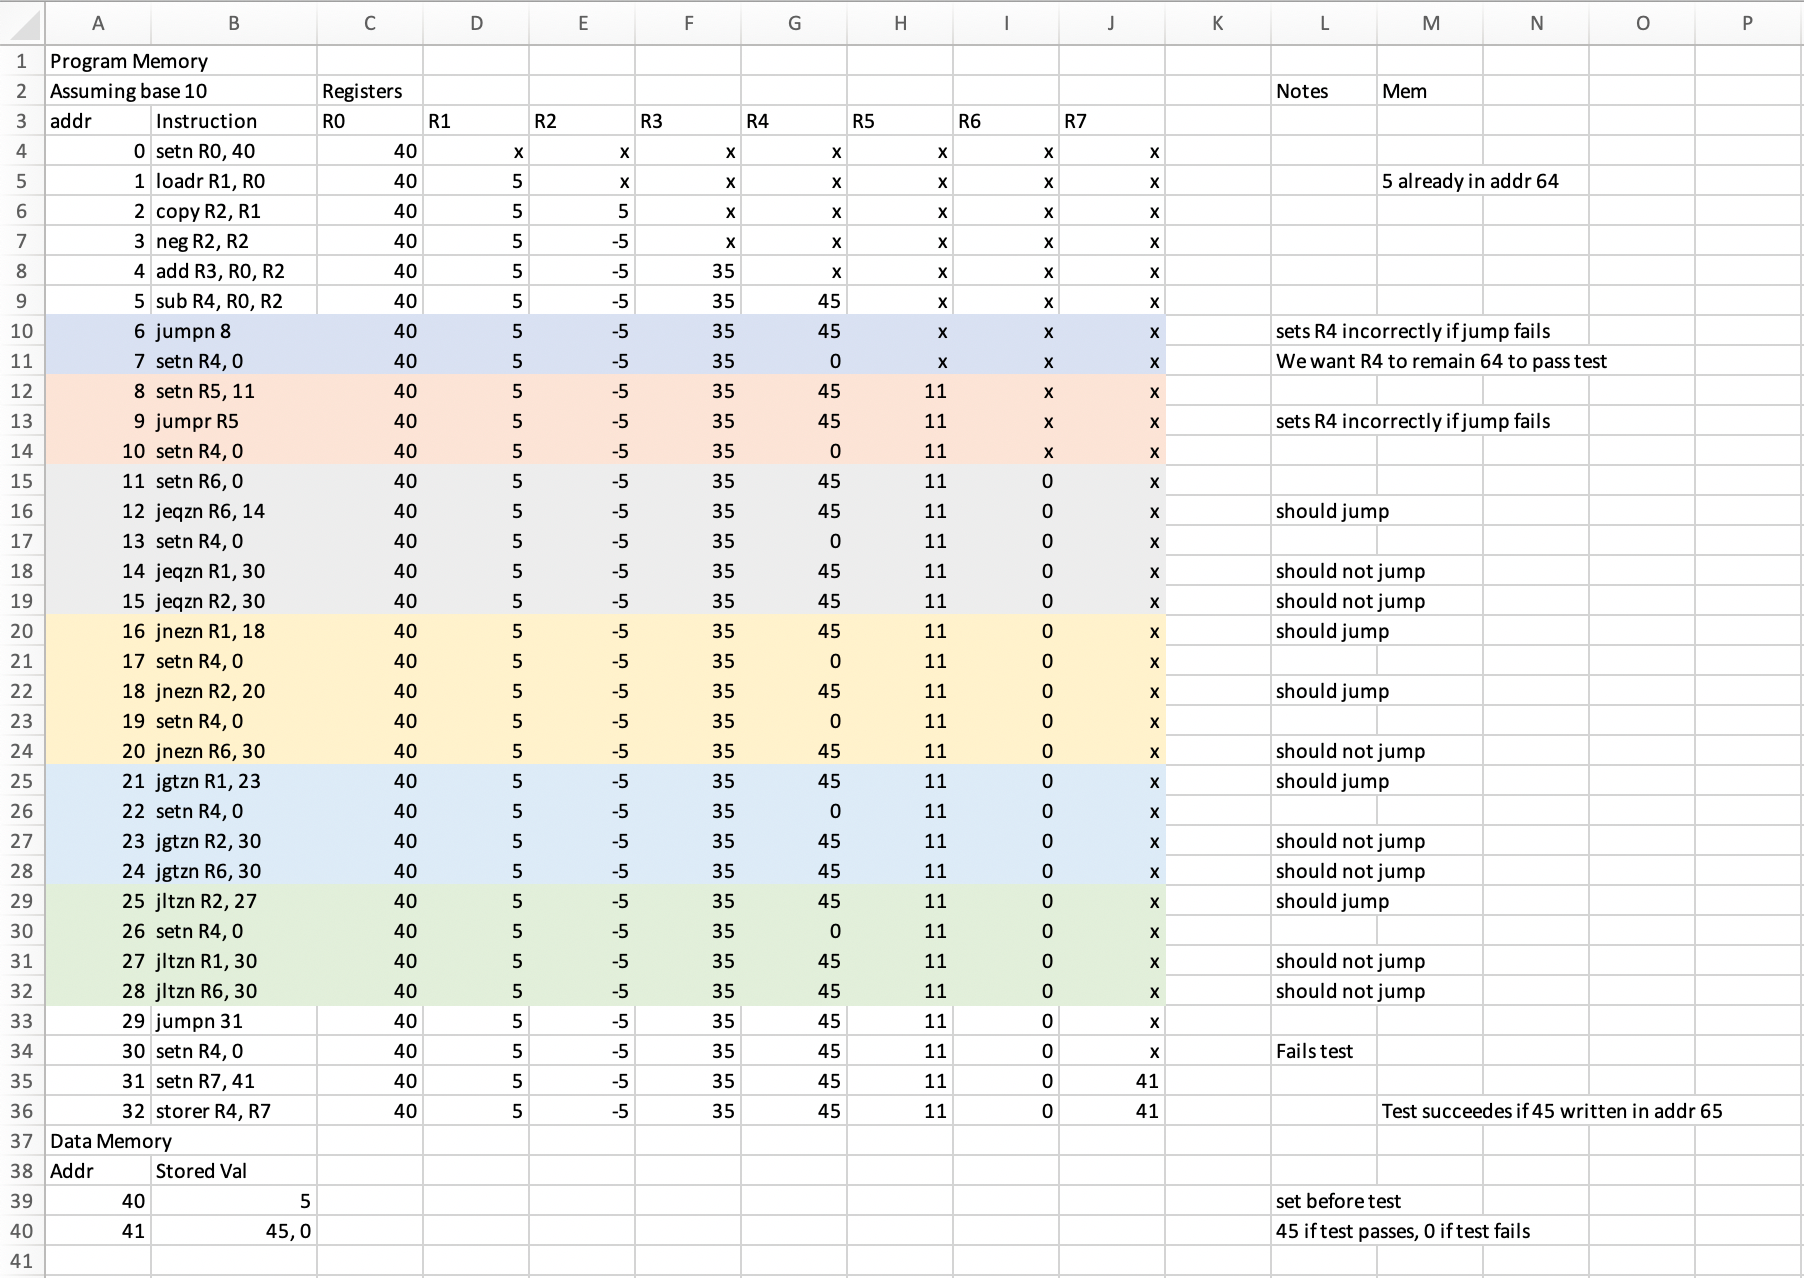
\includegraphics[width=16cm]{HMMMTestvectors.png}
        % replace this with actual drawn version
        \caption{The HMMMM Test Program, with annotated register states after each instruction}
        \end{center}
    \end{figure}
    \clearpage
    \section{Custom Leaf Cell: Tri-State Buffer}
    \subsection{Schematic}
    \begin{figure}[H]
        \begin{center}
        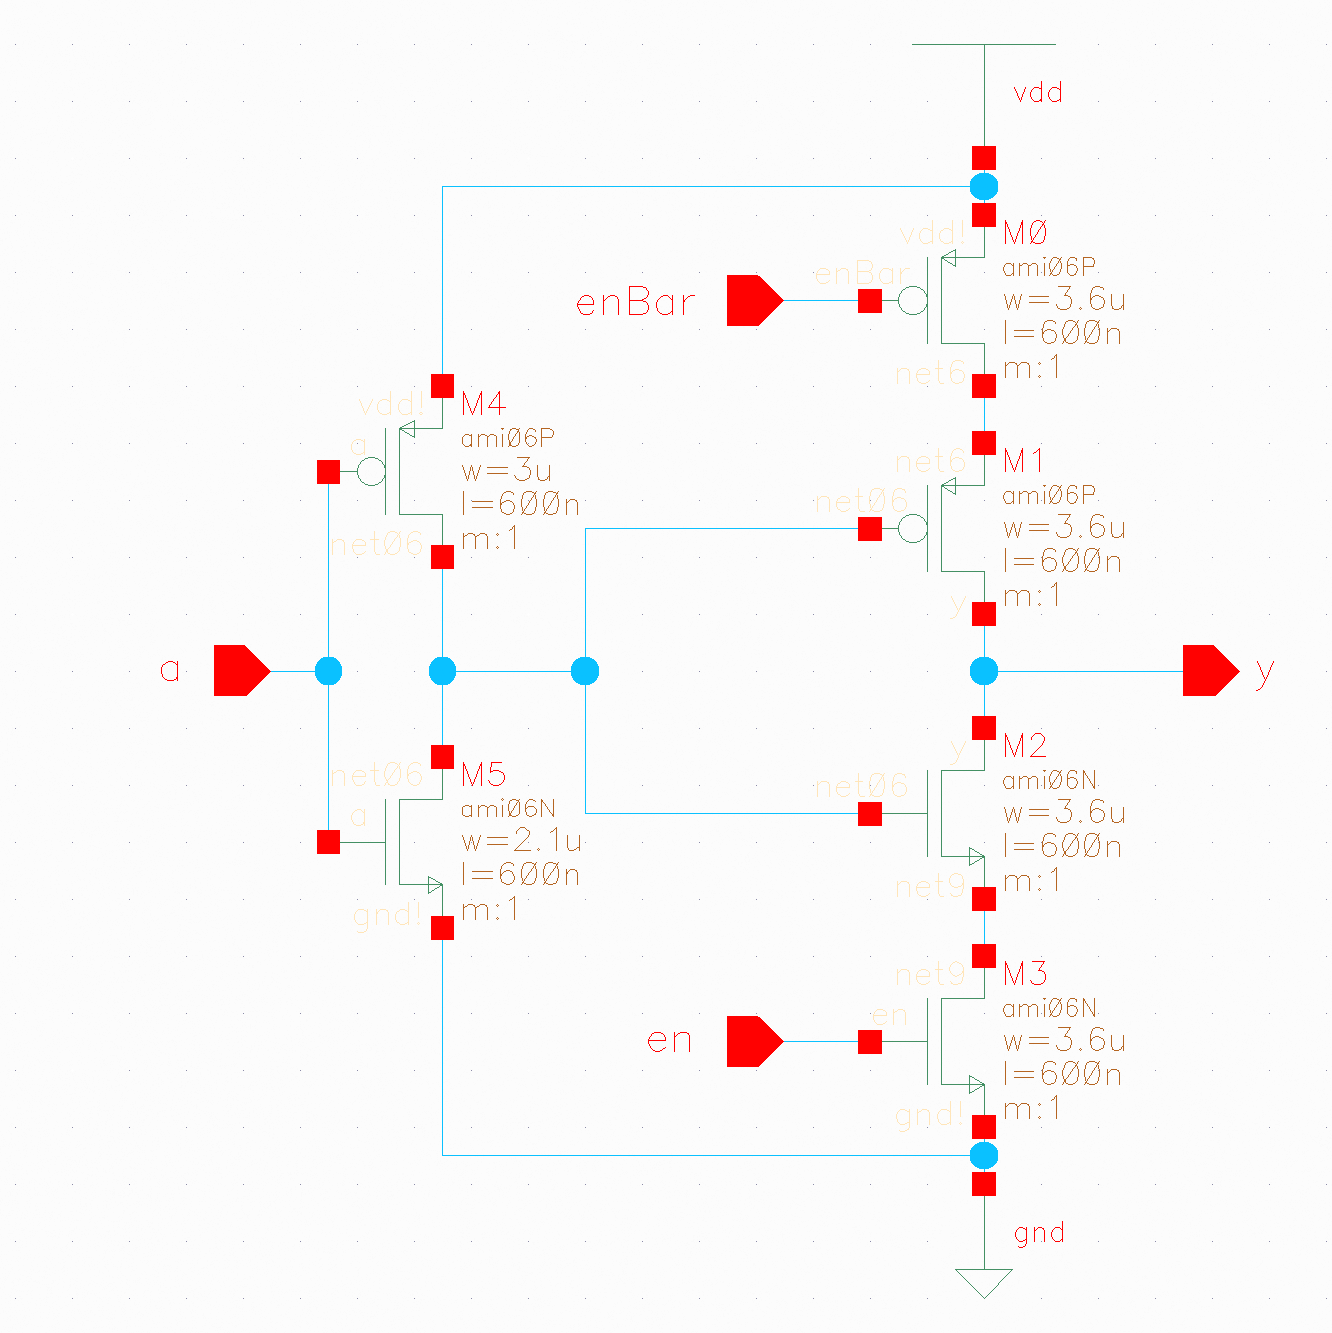
\includegraphics[width=16cm]{HMMMTristateSchematic.png}
        % replace this with actual drawn version
        \caption{Schematic for the custom tri-state buffer leaf cell}
        \end{center}
    \end{figure}
    \subsection{Symbol}
    \begin{figure}[H]
        \begin{center}
        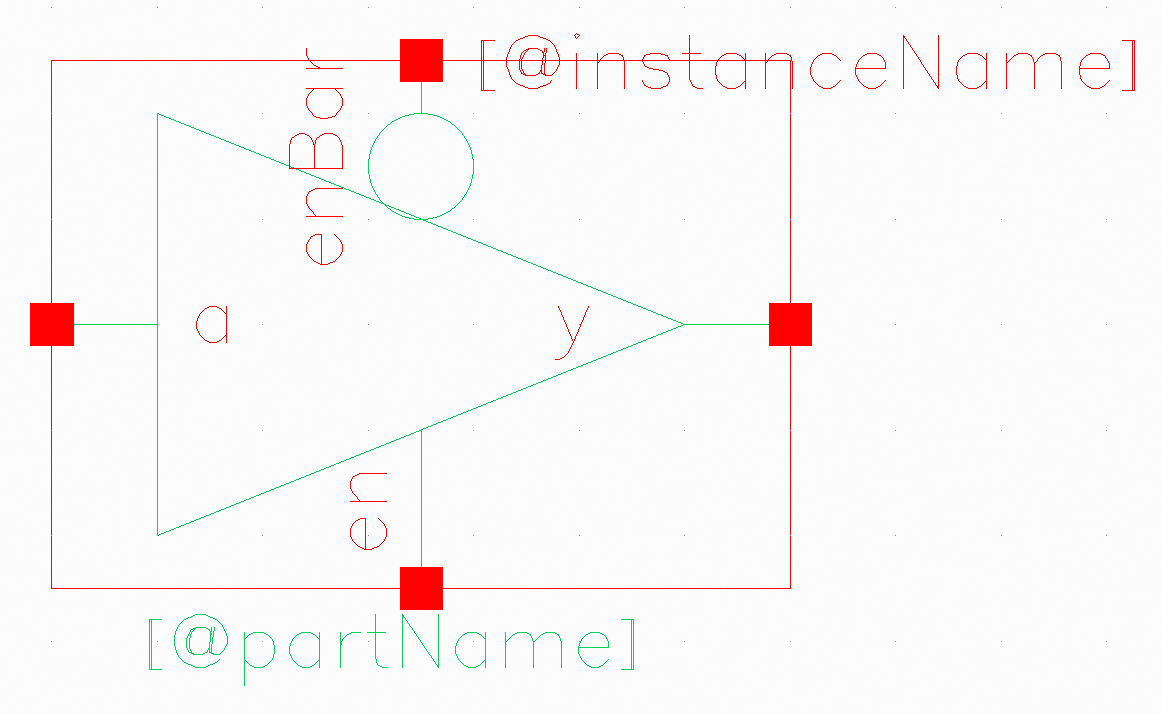
\includegraphics[width=16cm]{HMMMTristateSymbol.png}
        % replace this with actual drawn version
        \caption{Symbol for the custom tri-state buffer leaf cell}
        \end{center}
    \end{figure}
    \subsection{Layout}
    \begin{figure}[H]
        \begin{center}
        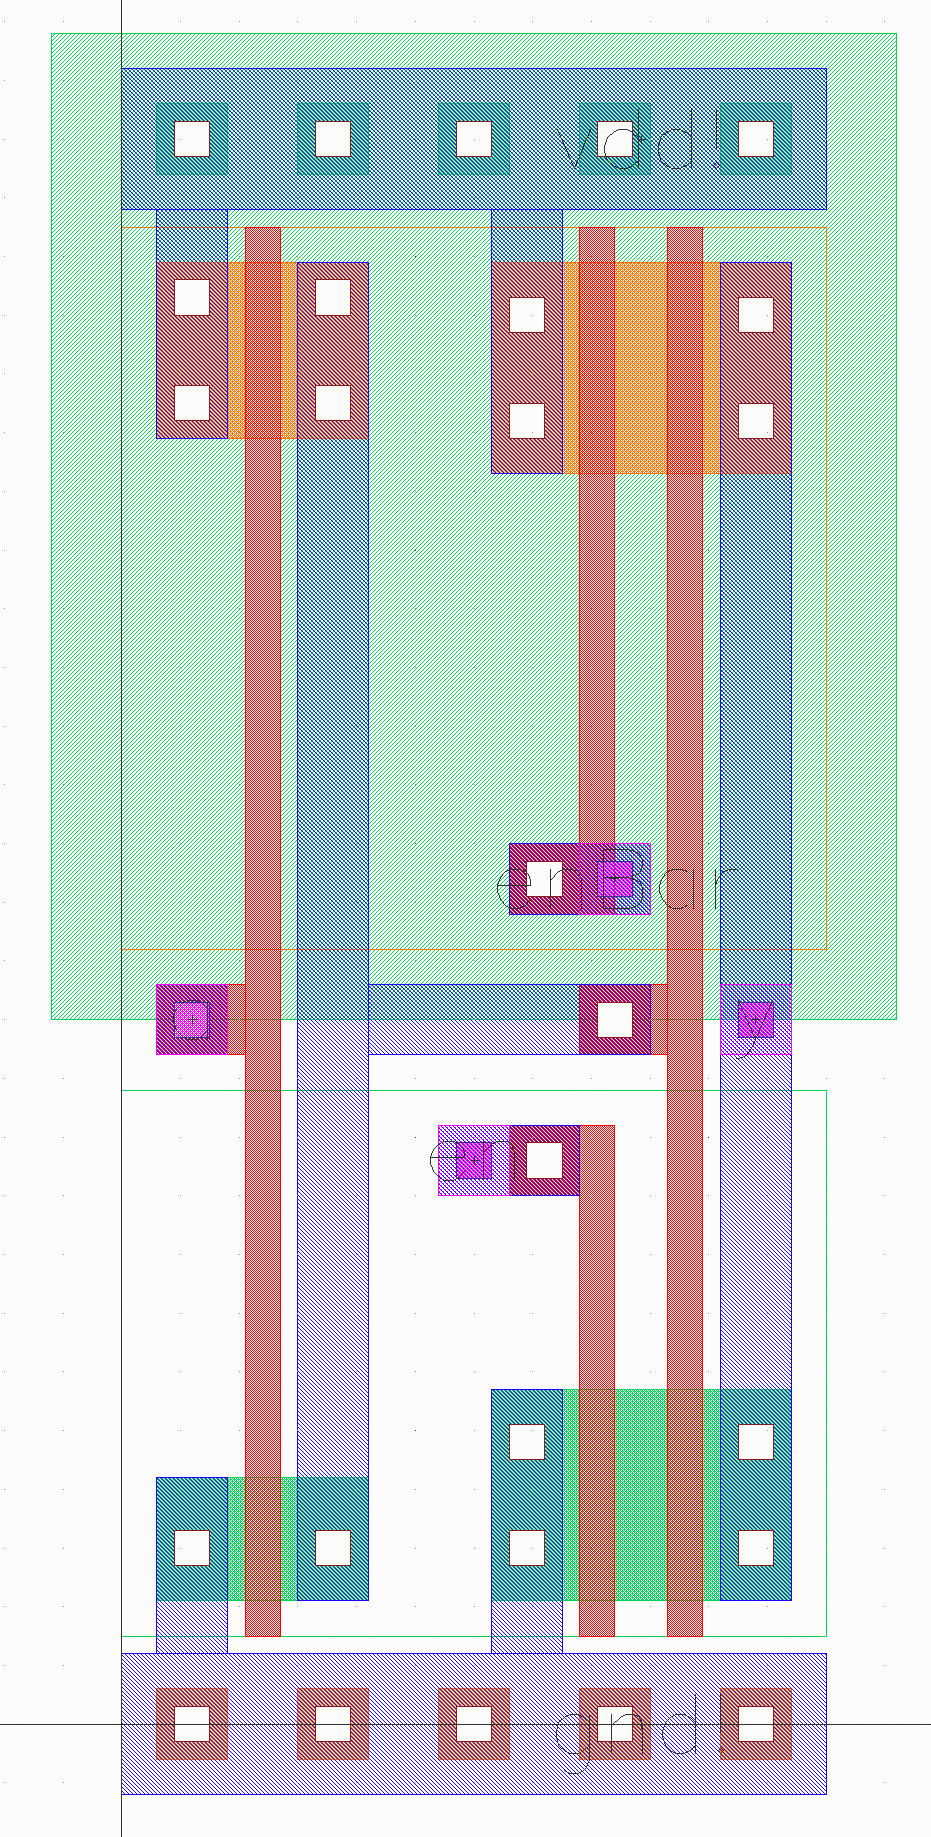
\includegraphics[width=10cm]{HMMMTristateLayout.png}
        % replace this with actual drawn version
        \caption{Layout for the custom tri-state buffer leaf cell}
        \end{center}
    \end{figure}
    \section{Layouts}
    \subsection{Controller}
    \begin{figure}[H]
        \begin{center}
        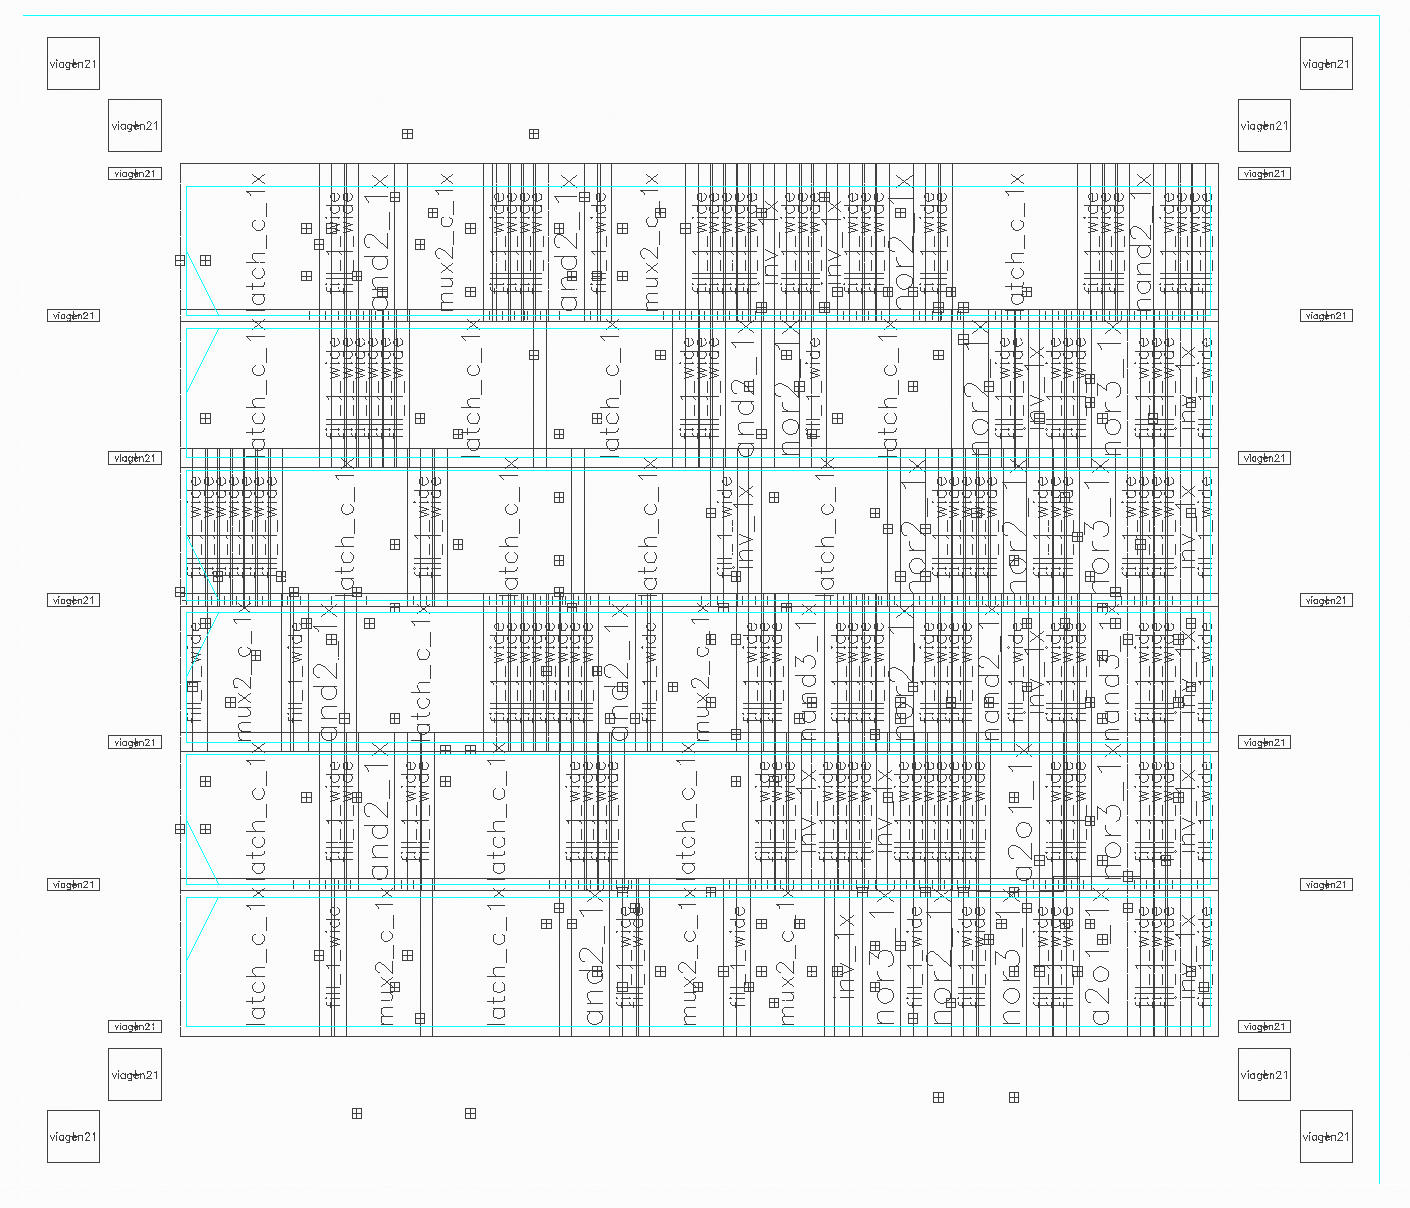
\includegraphics[width=16cm]{HMMMController.png}
        % replace this with actual drawn version
        \caption{Layout image of the HMMM Controller. Each named block denotes a sub-cell}
        \end{center}
    \end{figure}
    \subsection{Datapath}
    \begin{figure}[H]
        \begin{center}
        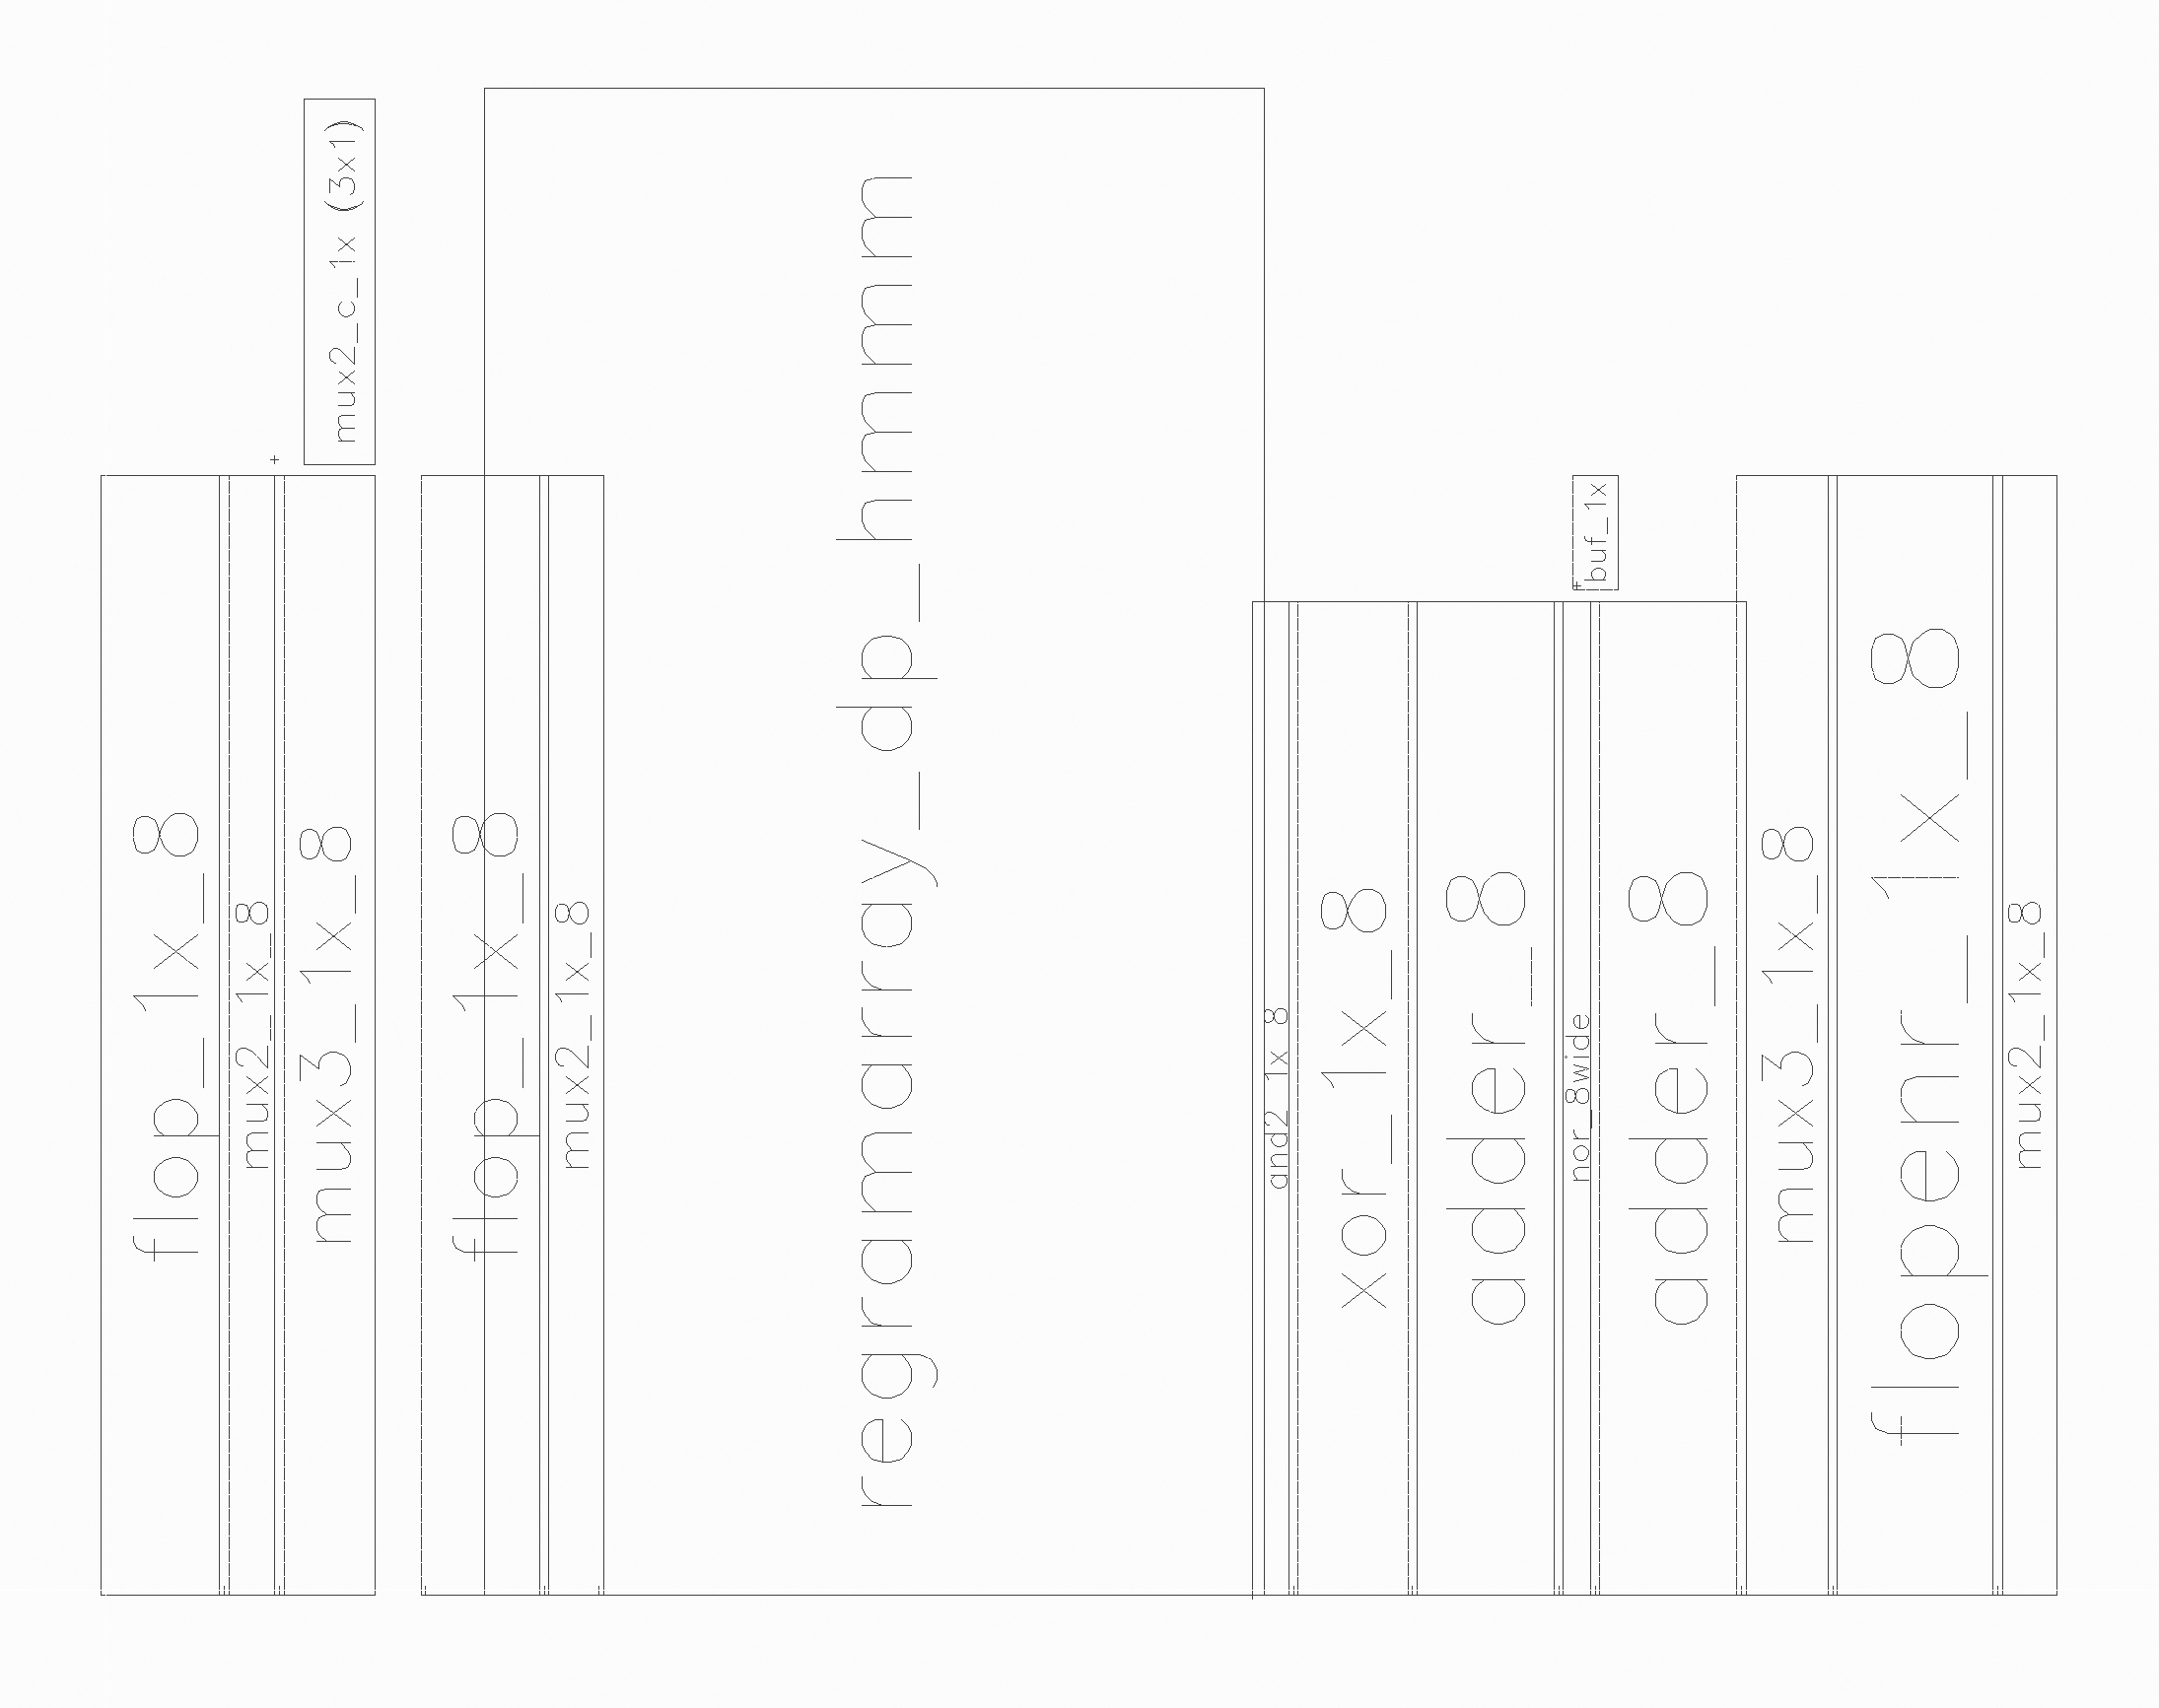
\includegraphics[width=16cm]{HMMMDatapath.png}
        % replace this with actual drawn version
        \caption{Layout image of the HMMM datapath. Each named block denotes a sub-cell}
        \end{center}
        \label{fig:layoutimages}
    \end{figure}

\end{appendices}
%label things

\end{document}

%TODO: discuss custom leaf cell

%TODO: include code
